The previous chapter highlighted the important structure of deep neural networks
and the empirical risk used to train them:
\begin{itemize}

\item \textbf{Sum structure \& noise:} Given a model $f_{\vtheta}$, a convex
  loss function $\ell$, and a dataset $\sD$, the empirical risk is an average
  over per-datum losses. Each of these losses is identically computed by feeding
  a datum through the model and the loss function. Batching these computations
  allows to efficiently evaluate them in parallel. Doing so on only a random
  subset of data---a mini-batch---reduces computational cost in exchange for
  noise.

\item \textbf{Probabilistic interpretation:} For specific loss functions, which
  include regression and softmax classification, empirical risk minimization can
  be interpreted as maximum likelihood---or maximum a posteriori---estimation
  where the model parameterizes a likelihood distribution
  $q(\giventhat{\vy}{f_{\vtheta}(\vx)})$.

\item \textbf{Layer-structure \& modularity:} Neural networks consist of layers,
  or modules, which are glued together by function composition. Backpropagation
  abstract the differentiation by the composition of the module-level
  derivatives, which simplifies supporting new operations and hides the
  complexity of AD from practitioners.
\end{itemize}
Popular ML libraries allow for efficient and automated gradient computation, but
combine AD and batching in a way that allows to support more general computation
graphs than the empirical risk. However, the added optimization complicates
efficiently assessing the empirical risk's per-sample structure, and
higher-order information which requires slightly more flexible AD operations,
like matrix-Jacobian products.

This chapter motivates why relying solely on the gradient has limitations,
and---based on structure in the empirical risk---proposes quantities in the form
of higher-order information that go beyond the gradient. It starts by presenting
currently popular deep learning optimization methods
(\Cref{sec:background::PopularOptimizers}) which rely heavily on the average
mini-batch gradient provided through AD in ML libraries. While training
algorithms that use more information than the gradient have been historically
mostly unexplored---because the quantities required are not as optimized and
automated as gradient computations---they have exciting promises.

Second-order methods (\Cref{sec:background::SecondOrderOptimization}) use more
information than just the gradient. They are known to improve over first-order
methods in ``classic'' optimization problems (convex optimization, general
linear models). They incorporate curvature information in form of the Hessian
(\Cref{sec:background::NewtonMethodAndHessian}), or PSD approximations thereof,
such as the generalized Gauss-Newton (\Cref{sec:background::ggn}) and Fisher
information matrix (\Cref{sec:background::naturalGradientDescent}).

While optimization methods for neural networks are one main application in deep
learning, there are other applications to quantities beyond the gradient.
\Cref{sec:background:moreApplications} highlights additional use cases which
underline the relevance of such information beyond optimization.
\Cref{chap:cockpit} presents another use case focused on improving the
training of neural networks.

\section{Popular Deep Learning
  Optimizers}\label{sec:background::PopularOptimizers}
\begin{figure*}[!p]
  \centering
  \begin{minipage}[t]{0.495\linewidth}
    \begin{updaterule}[\textbf{SGD~\cite{robbins1951stochastic}}]\label{opt:background::SGD}
      \begin{align*}
        \vtheta_{t+1} &= \vtheta_t - \eta \vg_{\sB_t}(\vtheta_t)
                        \shortintertext{with}
        &\text{learning rate $\eta \in \sR^+$}
      \end{align*}
    \end{updaterule}
    \vspace{-1.1ex}
    \begin{updaterule}[\textbf{Momentum~\cite{polyak1964some}}]\label{opt:background::Momentum}
      \begin{align*}
        \vtheta_{t+1} &= \vtheta_t - \vv_{t}
                        \shortintertext{where}
                        \vv_t &= \rho \vv_{t-1} + \eta \vg_{\sB_t}(\vtheta_t)
                                \shortintertext{with}
        &\text{learning rate $\eta \in \sR^+$}
        \\
                      &\text{momentum factor $\rho \in [0;1)$}
        \\
                      &\text{initial momentum $\vv_{0} \in \sR^{D}$}
      \end{align*}
    \end{updaterule}
    \vspace{-1.1ex}
    \begin{updaterule}[\textbf{NAG~\cite{nesterov1983method}}]\label{opt:background::NAG}
      \begin{align*}
        \vtheta_{t+1} &= \vtheta_t - \vv_{t}
                        \shortintertext{where}
                        \vv_t &= \rho \vv_{t-1} + \eta \vg_{\sB_t}(\vtheta_t - \rho \vv_{t-1})
                                \shortintertext{with}
        &\text{learning rate $\eta \in \sR^+$}
        \\
                      &\text{momentum factor $\rho \in [0;1)$}
        \\
                      &\text{initial momentum $\vv_{0} \in \sR^{D}$}
      \end{align*}
    \end{updaterule}
    \vspace{-1.1ex}
    \begin{updaterule}[\textbf{AdaGrad~\cite{duchi2011adaptive}}]\label{opt:background::AdaGrad}
      \begin{align*}
        \vtheta_{t+1} &= \vtheta_t - \eta \vg_{\sB_t}(\vtheta_t) \oslash (\vs_{t}^{\circ \nicefrac{1}{2}} + \epsilon \vone)
                        \shortintertext{where}
                        \vs_t &= \vs_{t-1} + (\vg_{\sB_t}(\vtheta_t))^{\circ 2}
                                \shortintertext{with}
        &\text{learning rate $\eta \in \sR^+$}
        \\
                      &\text{divide-by-zero safe guard $\epsilon \in \sR^+$}
        \\
                      &\text{initial $\vs_{0} \in \sR^{D}$}
      \end{align*}
    \end{updaterule}
    \vspace{-1.1ex}
    \begin{updaterule}[\textbf{RMSProp~\cite{tieleman2012lecture}}]\label{opt:background::RMSProp}
      \begin{align*}
        \vtheta_{t+1} &= \vtheta_t - \eta \vg_{\sB_t}(\vtheta_t) \oslash (\vs_{t}^{\circ \nicefrac{1}{2}} + \epsilon \vone)
                        \shortintertext{where}
                        \vs_t &= \rho \vs_{t-1} + (1-\rho) (\vg_{\sB_t}(\vtheta_t))^{\circ 2}
                                \shortintertext{with}
        &\text{learning rate $\eta \in \sR^+$}
        \\
                      &\text{decay rate $\rho \in [0;1)$}
        \\
                      &\text{divide-by-zero safe guard $\epsilon \in \sR^+$}
        \\
                      &\text{initial $\vs_{0} \in \sR^{D}$}
      \end{align*}
    \end{updaterule}
  \end{minipage}
  \hfill
  \begin{minipage}[t]{0.495\linewidth}
    \begin{updaterule}[\textbf{Adadelta~\cite{zeiler2012adadelta}}]\label{opt:background::Adadelta}
      \begin{align*}
        \vtheta_{t+1} &= \vtheta_t - \eta \vDelta_{t}
                        \shortintertext{where}
                        \vDelta_{t} &= (\vd_{t} + \epsilon \vone)^{\circ \nicefrac{1}{2}} \oslash (\vs_{t} + \epsilon \vone)^{\circ \nicefrac{1}{2}} \odot \vg_{\sB_t}(\vtheta_t)
                                      \shortintertext{\quad \ \, where}
        &\vs_t = \rho \vs_{t-1} + (1-\rho) (\vg_{\sB_t}(\vtheta_t))^{\circ 2}
        \\
                      &\vd_t = \rho \vd_{t-1} + (1-\rho) \vDelta_{t-1}^{\circ 2}
                        \shortintertext{with}
                                    &\text{learning rate $\eta \in \sR^+$}
        \\
                      &\text{decay rate $\rho \in [0;1)$}
        \\
                      &\text{divide-by-zero safe guard $\epsilon \in \sR^+$}
        \\
                      &\text{initial $\vs_{0}, \vd_{0}, \vDelta_{0} \in \sR^{D}$}
      \end{align*}
    \end{updaterule}
    \vspace{-1.1ex}
    \begin{updaterule}[\textbf{Adam~\cite{kingma2015adam}}]\label{ex:background::Adam}
      \begin{align*}
        \vtheta_{t+1} &= \vtheta_t - \eta \vmhat_{t}\oslash ( \vvhat_{t}^{\circ \nicefrac{1}{2}} + \epsilon \vone)
                        \shortintertext{where}
                        \vmhat_{t} &= \nicefrac{\vm_{t}}{(1 - \beta_{1}^{t})}
                                     \shortintertext{\quad \ \, where}
        &\vm_{t} = \beta_1 \vm_{t-1} + (1 - \beta_{1}) \vg_{\sB_t}(\vtheta_{t})
        \\
        \vvhat_t &= \nicefrac{\vv_t}{(1 - \beta_2^t)}
                   \shortintertext{\quad \ \, where}
                                   &\vv_t = \beta_2 \vv_{t-1} + (1 - \beta_2) (\vg_{\sB_t}(\vtheta_t))^{\circ 2}
                                     \shortintertext{with}
        &\text{learning rate $\eta \in \sR^+$}
        \\
                      &\text{decay rates $\beta_1, \beta_2 \in [0;1)$}
        \\
                      &\text{divide-by-zero safe guard $\epsilon \in \sR^+$}
        \\
                      &\text{initial $\vm_{0}, \vv_{0}, \in \sR^{D}$}
      \end{align*}
    \end{updaterule}
    \vspace{-1.1ex}
    \begin{updaterule}[\textbf{AMSGrad~\cite{reddi2018on}}]\label{opt:background::AMSGrad}
      \begin{align*}
        \vtheta_{t+1} &= \vtheta_t - \eta \vmhat_{t}\oslash ( \vvhat_{t}^{\circ \nicefrac{1}{2}} + \epsilon \vone)
                        \shortintertext{where}
                        \vmhat_{t} &= \nicefrac{\vm_{t}}{(1 - \beta_{1}^{t})}
                                     \shortintertext{\quad \ \, where}
        &\vm_{t} = \beta_1 \vm_{t-1} + (1 - \beta_{1}) \vg_{\sB_t}(\vtheta_{t})
        \\
        \vvhat_t &= \nicefrac{\vv_t}{(1 - \beta_2^t)}
                   \shortintertext{\quad \ \, where}
                                   &\vv_t = \max( \beta_2 \vv_{t-1} + (1 - \beta_2) (\vg_{\sB_t}(\vtheta_t))^{\circ 2}, \vv_{t-1})
                                     \shortintertext{with}
        &\text{learning rate $\eta \in \sR^+$}
        \\
                      &\text{decay rates $\beta_1, \beta_2 \in [0;1)$}
        \\
                      &\text{divide-by-zero safe guard $\epsilon \in \sR^+$}
        \\
                      &\text{initial $\vm_{0}, \vv_{0}, \in \sR^{D}$}
      \end{align*}
    \end{updaterule}
  \end{minipage}
  \vspace{-1ex}
  \caption{\textbf{Popular deep learning optimizers rely on the average
      mini-batch gradient.} At iteration $t$, they incorporate information in
    form of the mini-batch average gradient $\vg_{\sB_t}$. This is a
    representative subset of popular methods; see \cite{schmidt2021descending}
    for a more complete
    overview.}\label{fig:background::popularDeepLearningOptimizers}
\end{figure*}

%%% Local Variables:
%%% mode: latex
%%% TeX-master: "../../thesis"
%%% End:


\Cref{sec:background::SupervisedLearning} formulates learning as minimizing the
empirical risk, for which an optimization algorithm seeks to find a solution.
Deep learning optimizers are iterative: they start from an initial parameter
$\vtheta_{0}$ and aim to improve the parameters in iterations, leading
to a trajectory $\vtheta_{0}, \vtheta_{1}, \dots$ in parameter space. An
iteration is described by an update rule $\gM: \vtheta_{t} \mapsto
\vtheta_{t+1}$ that relies on internal states of the optimizer from the
observation history $H_t$, local observations at the current iterate
$\vtheta_t$, and hyperparameters $\phi_t$~\cite{choi2020on}. The next iterate
results from a simplified optimization problem where the actual objective is
replaced by a computationally cheap approximation. Often, this direction is
further adapted by outer-loop mechanisms, like line searches, or hyperparameters
that require manual tuning to achieve good performance.

The update quality is influenced by the quality of the local approximation.
Computing exact information about the objective $\gL_{\sD}$ is expensive, but
yields a more accurate local proxy. Due to the large-scale nature of deep
learning, algorithms only rely on stochastic information from a mini-batch
$\sB_t$ in form of the mini-batch loss $\gL_{\sB_t}$
(\Cref{sec:background::MiniBatching}). In addition to locality, noise further
complicates deriving a precise local approximation.

\subsubsection{Stochastic Gradient Descent}
One of the most popular methods, according to
\Cref{fig:background::ArxivMentions}, is stochastic gradient descent (\sgd,
\citep{robbins1951stochastic}). Its update derives from
\begin{subequations}
  \begin{align}
    \gM:\qquad
    \vtheta_{t+1}
    =
    \argmin_{\vtheta} m_{\vtheta_t}(\vtheta)
    =
    \vtheta_t - \eta \vg_{\sB_t}(\vtheta_t)
  \end{align}
  where $m_{\vtheta_t}(\vtheta)$ is a first-order Taylor around the current
  iterate $\vtheta_t$ based on the mini-batch gradient, regularized by a quadratic
  $L_2$ penalty to discourage large steps with a learning rate $\eta$,
  \begin{align}\label{eq:background::SGDLocalApproximation}
    m_{\vtheta_t}(\vtheta)
    =
    \gL_{\sB_t}(\vtheta_t)
    +
    {\vg_{\sB_t}(\vtheta_t)}^{\top}
    (\vtheta - \vtheta_t)
    +
    \frac{1}{2 \eta}
    \lVert \vtheta - \vtheta_t \rVert_2^2
  \end{align}
\end{subequations}
This leads to \Cref{opt:background::SGD}, which updates the parameters with the
scaled negative mini-batch gradient. The negative gradient also corresponds to
the direction of steepest descent, \ie along which the loss decreases most
rapidly around $\vtheta_t$ (see
\Cref{sec:background::naturalGradientDescent,eq:background::negativeGradientSteepestDescent}).

\subsubsection{Momentum Methods (Incorporating Past Knowledge)}

The descent direction in \sgd becomes poorer as the mini-batch gradient is
subject to more noise. Incorporating previous gradient observations can help
reduce noise and find a better descent direction~\cite[][Chapter
8.3]{goodfellow2016deep}. From a physical interpretation, the optimizer builds
up a velocity (referred to as \emph{momentum}) that is adapted with new gradient
observation. Two variations are the heavy ball~\cite{polyak1964some} and
Nesterov~\cite{nesterov1983method} momentum methods
(\Cref{opt:background::Momentum,opt:background::NAG}). Another intuition for
momentum is that it suppresses \sgd's oscillating behavior in the presence of
two directions with differing curvature by averaging out gradients that point in
opposite directions (see \eg central panel of \Cref{cockpit::fig:LINE}).

\subsubsection{Adaptive Methods (Per-parameter Learning Rate)}

Adaptive methods like AdaGrad~\cite{duchi2011adaptive},
RMSProp~\cite{tieleman2012lecture}, Adadelta~\cite{zeiler2012adadelta},
Adam~\cite{kingma2015adam}~\&~AMSGrad~\cite{reddi2018on} keep a learning rate
for each parameter that is adapted over time. This rescaling is driven by the
elementwise square of the mini-batch gradient, $\vg_{\sB_t}(\vtheta_t)^{\odot
  2}$
(\Cref{opt:background::AdaGrad,opt:background::RMSProp,opt:background::Adadelta,ex:background::Adam,opt:background::AMSGrad}).
These algorithms use this quantities in different ways, motivated by
shortcomings of predecessors (\eg too aggressive learning rate
shrinking~\cite{tieleman2012lecture,zeiler2012adadelta} and convergence
problems~\cite{reddi2018on}).

\subsubsection{No Clear Winner \& Mini-batch Gradient as Central Object}

\Cref{fig:background::popularDeepLearningOptimizers} summarizes the update rules
of the above optimization methods. Their update rules to derive $\vtheta_{t+1}$
rely on three ingredients:
\begin{itemize}
\item The history of iterates $\{\vtheta_{t'}\}_{t'=0}^{t}$
\item The history of gradients\sidenote{%
    One mild exception is Nesterov momentum (\Cref{opt:background::NAG}). It
    relies on the ``lookahead'' gradient history rather than the gradient
    history of iterates.}%
  $\{\vg_{\sB_{t'}}(\vtheta_{t'})\}_{t'=0}^{t}$

\item The history of elementwise gradient squares
  $\{\vg_{\sB_{t'}}(\vtheta_{t'})^{\odot 2}\}_{t'=0}^{t}$
  % , which can be derived from the gradient history
\end{itemize}
In summary, the main ingredient in all of these methods is the average
mini-batch gradient (and its elementwise square). Their updates are cheap and
only require computation of average mini-batch gradients, as efficiently
provided by AD in popular ML libraries
(\Cref{sec:background::GradientBackpropagation}):
\begin{align}\label{eq:background::PopularOptimizers}
  \begin{split}
    \gM
    &=
      \gM(
      H_t,
      \phi_t)
    \\
    \text{with}\qquad
    H_t
    &=
      \left\{\vtheta_{t'}\right\}_{t'=0}^{t},
      \cup
      \left\{\vg_{\sB_{t'}}(\vtheta_{t'}) \right\}_{t'=0}^{t},
      \cup
      \left\{\vg_{\sB_{t'}}(\vtheta_{t'})^{\odot 2} \right\}_{t'=0}^{t},
  \end{split}
\end{align}
While the mentioned methods are a representative subset of popular algorithms,
there are more than one hundred algorithms with structurally similar update
rules (see Table 2 in~\cite{schmidt2021descending} and references therein). Some
adaptive methods like Adam and RMSProp contain simpler methods like SGD and
Momentum as special cases~\cite{choi2020on}. Therefore, they should, in
principle, be able to perform better. However, recent work that compares deep
learning optimizers through benchmarks to identify the best-performing method
finds that the currently existing methods perform quite
similarly~\cite{schmidt2021descending}.

One reason why newly developed optimizers of the structure
\Cref{eq:background::PopularOptimizers} seem to not be able to clearly improve
over existing methods could be that their update rules are constrained to using
the average gradient, as it is readily available in software. To overcome these
limitations, it might be helpful to study the potential of methods that leverage
information beyond the gradient. Second-order optimization incorporate curvature
information and represent the state-of-the art in ``classical'' optimization
problems (convex optimization, generalized linear models). Noise-reduction
methods focus on improving the gradient estimator $\vg_{\sB_t}$ by reducing its
variance through per-sample information. The rest of this chapter provides
definitions for the information used by such methods, and provides additional
motivation for them by showcasing applications outside optimization.

%%% Local Variables:
%%% mode: latex
%%% TeX-master: "../thesis"
%%% End:


\section{Second-order
  Optimization}\label{sec:background::SecondOrderOptimization}
Second-order methods iteratively optimize an objective $\gL(\vtheta): \sR^{D}
\to \sR$ using a local quadratic approximation $\gL(\vtheta) \approx
m_{\vtheta_t}(\vtheta)$ around the current point $\vtheta_t$ after $t$
iterations,
\begin{subequations}
  \begin{align}\label{eq:background::localQuadraticApproximation}
    m_{\vtheta_t}(\vtheta)
    =
    a(\vtheta_t)
    +
    {\vb(\vtheta_t)}^{\top}(\vtheta - \vtheta_t)
    +
    \frac{1}{2}
    (\vtheta - \vtheta_t)^{\top}
    \mC(\vtheta_t)
    (\vtheta - \vtheta_t)\,,
  \end{align}
  with an offset $a(\vtheta_t) \in \sR$, a slope vector $\vb(\vtheta_t) \in
  \sR^{D}$, and a curvature matrix $\mC(\vtheta_t) \in \sR^{D \times D}$. As
  described in \Cref{sec:background::PopularOptimizers}, the next iterate
  $\vtheta_{t+1}$ is obtained by minimizing the local approximation. For this
  proxy to possess a minimum, the curvature matrix $\mC(\vtheta_t)$ must be PD.
  Then, \Cref{eq:background::localQuadraticApproximation} is minimized by
  \begin{align}\label{eq:background::SecondOrderUpdateInverseCurvature}
    \vtheta_{t+1}
    =
    \argmin_{\vtheta} m_{\vtheta_t}(\vtheta)
    =
    \vtheta_t - {\mC(\vtheta_t)}^{-1} \vb(\vtheta_t)\,.
  \end{align}
  This update is computationally challenging, because the size of the curvature
  matrix is quadratic in $D$ and generally infeasible to store. Additionally,
  the computational complexity of matrix inversion scales cubically in $D$.
  These problems can somewhat be addressed by approximately solving the linear
  system
  \begin{align}\label{eq:background::SecondOrderMethodsLinearSystem}
    \mC(\vtheta_t) \vtheta_{t+1} = - \vb(\vtheta_t)
  \end{align}
\end{subequations}
for $\vtheta_{t+1}$. This can be done with iterative solvers, such as CG, which
only require matrix-vector products with $\mC(\vtheta_t)$, which can often be
implemented without expanding the matrix representation in memory.

The first-order methods from \Cref{sec:background::PopularOptimizers} circumvent
these issues by using a diagonal---and often quite crude---curvature
approximation that is cheap to store and invert (see~\cite{choi2020on} for an
overview). \Eg, \sgd's local approximation,
\Cref{eq:background::SGDLocalApproximation}, uses $\nicefrac{1}{2\eta}\mI$ as
curvature matrix. The following sections introduce common curvature matrices for
local approximations of empirical risks.

\subsection{Newton's Method \& the Hessian
  Matrix}\label{sec:background::NewtonMethodAndHessian}
The Taylor series provides a meaningful local approximation of an analytic
function. Its expansion up to second-order is
\begin{align}
  \begin{split}
    \gL(\vtheta)
    &=
      \underbrace{
      \gL(\vtheta_t)
      }_{a(\vtheta_t)}
      +
      {
      \underbrace{
      \grad{\vtheta_{t}}\gL(\vtheta_t)
      }_{\vb_{\vtheta_t}}
      }^{\top}
      ( \vtheta - \vtheta_t)
    \\
    &\phantom{= }
      +
      \frac{1}{2}
      {( \vtheta - \vtheta_t)}^{\top}
      \underbrace{
      \gradsquared{\vtheta_t}\gL(\vtheta_t)
      }_{\mC(\vtheta_t)}
      ( \vtheta - \vtheta_t)
      +
      \gO\left( {(\vtheta - \vtheta_t)}^{3} \right)
  \end{split}
\end{align}
where $\gO((\vtheta - \vtheta_t)^{3})$ denotes polynomial terms in the
components of $\vtheta - \vtheta_t$ of cubic order and above. This reveals the
objective's Hessian $\gradsquared{\vtheta_t}\gL(\vtheta_t)$, which collects its
second-order partial derivatives in a matrix
${[\gradsquared{\vtheta_t}\gL(\vtheta_t)]}_{i,j} = \nicefrac{\partial^2
  \gL(\vtheta_t)}{\partial {[\vtheta_t]}_i \partial {[\vtheta_t]}_j}$, as
curvature matrix.

\begin{definition}[\textbf{Hessian}]\label{def:background::Hessian}
  Let $b: \sR^D \to \sR; \va \mapsto b(\va)$ be a differentiable
  vector-to-scalar function. The Hessian $\gradsquared{\va} b \in \sR^{D\times
    D}$ of $b$ \wrt $\va$ is a symmetric matrix containing the second-order
  partial derivatives
  \begin{align}
    \label{eq:background::HessianVectorToScalar}
    \gradsquared{\va}b = \frac{\partial^2 b}{\partial \va \partial \va^{\top}}
    \qquad
    \text{with}
    \qquad
    [\gradsquared{\va}b]_{i,j} = \frac{\partial^2 b}{\partial \eva_i \partial \eva_j}
  \end{align}
  \Cref{hbp::def:generalizedHessian} generalizes this to the matrix/tensor case.
  The Hessian will often be denoted by $\mH$. \Eg $\mH_{\pdata}(\vtheta) :=
  \gradsquared{\vtheta} \gL_{\pdata}(\vtheta)$ for the Hessian of the population
  risk \Cref{eq:background::expectedRisk}, and $\mH_{\sD}(\vtheta) :=
  \gradsquared{\vtheta} \gL_{\sD}(\vtheta)$ for the Hessian of the empirical
  risk \Cref{eq:background::empiricalRisk} on a dataset $\sD$ (with $\sD =
  \Dtrain,\sB$ for the train loss and mini-batch Hessian).
\end{definition}

\marginnote[*-5]{%
  \begin{definition}[\textbf{Generalized
      Hessian}]\label{hbp::def:generalizedHessian}
    Let $\mB: \mathbb{R}^{n\times q} \to \mathbb{R}^{m \times p}$ be a twice
    differentiable matrix function. The \emph{Hessian} $\gradsquared{\mA} \mB(\mA)$
    is an $(mnpq \times nq)$ matrix defined by
    \begin{align}
      \label{hbp::equ:generalizedHessian}
      \begin{split}
        &\gradsquared{\mA} \mB(\mA)
        \\
        &= \jac_{\mA} \left[\jac_{\mA} \mB(\mA)\right]^\top
        \\
        &= \frac{
          \partial
          }{
          \partial (\vec \mA)^\top
          }
          \vec \left\{
          \left[
          \frac{\partial \vec \mB(\mA)}{\partial (\vec
          \mA)^\top}
          \right]^\top
          \right\}
      \end{split}
    \end{align}
    \citep[][Chapter 10.2]{magnus1999MatrixDifferentialCalculus} with
    flattening defined by \Cref{def:background::Flattening}. In
    element-wise notation, this is
    the matrix-stack of all output component Hessians
    \begin{align*}
      \gradsquared{\mA}
      \mB(\mA)
      =
      \begin{pmatrix}
        \gradsquared{\vec \mA} [\vec \mB]_1
        \\
        \gradsquared{\vec \mA} [\vec \mB]_2
        \\
        \vdots
        \\
        \gradsquared{\vec \mA} [\vec \mB]_{np}
      \end{pmatrix}\,,
    \end{align*}
    with the Hessian from \Cref{def:background::Hessian}.
  \end{definition}
  The tensor case is analogous but requires cluttered notation and is therefore
  omitted. Common forms for neural networks include vector-to-vector functions
  $f: \sR^m \to \sR^n, \vx \mapsto f(\vx)$ with
  \begin{align*}
    \gradsquared{\vx} f(\vx)
    =
    \frac{\partial^2 f(\vx)}{\partial \vx^\top \partial \vx}\,,
  \end{align*}
  where $\vx$ can be considered the input or bias vector if a linear layer. In
  details,
  \begin{align}
    \label{hbp::equ:HessianVectorToVector}
    \gradsquared{\vx} f(\vx)
    =
    \begin{pmatrix}
      \gradsquared{\vx} f_1(\vx)
      \\
      \vdots
      \\
      \gradsquared{\vx} f_m(\vx)
    \end{pmatrix}\,.
  \end{align}
  Others are matrix-to-vector mappings $f:\sR^{n\times q}\to \sR^m, \mX
  \to f(\mX)$ with
  \begin{align*}
    \gradsquared{\mX} f(\mX)
    =
    \frac{\partial}{\partial (\vec \mX)^\top}\frac{\partial f(\mX)}{\partial \vec \mX}\,,
  \end{align*}
  \eg with $\mX$ the weight of a linear layer.%
}

Newton's method uses the Hessian as curvature matrix.

\begin{updaterule}[\textbf{Newton's method (simplified)}]\label{opt:background::Newton}
  A Newton step is
  \begin{align}
    \vtheta_{t+1} = \vtheta_t - {\mH_{\sD}(\vtheta_t)}^{-1} \vg_{\sD}(\vtheta_t)
  \end{align}
  with the gradient and Hessian from
  \Cref{def:background::JacobianVectorVector,def:background::Hessian} (practical
  implementations vary and often introduce additional hyperparameters such as a
  learning rate, damping term, mini-batch size, \etc).
\end{updaterule}

Matrix-free multiplication with the Hessian~\cite{pearlmutter1994fast} can been
combined with CG to compute Newton steps via solving the linear system
\Cref{eq:background::SecondOrderMethodsLinearSystem}. This idea is known as
Hessian-free optimization~\cite{martens2010deep}.

While the Taylor expansion motivates using the Hessian as curvature matrix, it
leads to problems for non-convex functions like the empirical risk, as it is in
general indefinite. Therefore
\Cref{eq:background::SecondOrderUpdateInverseCurvature} does not have a
solution. In practice, PSD curvature matrices that are approximations of the
Hessian are popular substitutes for the Hessian to avoid this issue
(\Cref{sec:background::gn,sec:background::ggn,sec:background::naturalGradientDescent}).

\subsection{The Gauss-Newton Method \& Matrix}\label{sec:background::gn}

The Gauss-Newton (GN) method~\cite[chapter 6.3]{bottou2016machine} tackles the
nonlinear least squares regression task (\Cref{ex:background::Regression}) of
fitting a function $f_{\vtheta}$ to data in the form of vector-valued inputs
$\vx_n \in \sR^M$ and scalar-valued outputs $y_n \in \sR$ by minimizing the mean
squared error,
\begin{align}\label{eq:background::nonlinearLeastSquares}
  \minimize_{\vtheta} \gL(\vtheta)\,,
  \quad
  \text{where}
  \quad
  \gL(\vtheta)
  =
  \frac{1}{|\sD|}
  \sum_{(\vx_n, y_n) \in \sD}
  {(
  \underbrace{f_{\vtheta}(\vx_n)}_{:=f_n} - y_n
  )}^{2}\,,
\end{align}
The objective's gradient is
\begin{align}
  \label{eq:background::GradientNonlinearLeastSquares}
  \grad{\vtheta}\gL(\vtheta)
  =
  \frac{2}{|\sD|}
  \sum_{(\vx_n, y_n) \in \sD}
  {(\jac_{\vtheta} f_n)}^{\top}
  \left(
  f_n - y_{n}
  \right)\,,
\end{align}
with the Jacobian $\jac_{\vtheta} f_n \in \sR^{1 \times D}$
(\Cref{def:background::JacobianVectorVector}). The Hessian is
\begin{subequations}\label{eq:background::HessianDecompositionGaussNewtonResidual}
  \begin{align}
    \label{eq:background::HessianNonlinearLeastSquares}
    % \begin{split}
    \gradsquared{\vtheta} \gL(\vtheta)
    &=
      \frac{2}{|\sD|}
      \sum_{(\vx_n, y_n) \in \sD}
      {(\jac_{\vtheta}f_n)}^{\top}
      \jac_{\vtheta}f_n
      % \\
      % &\phantom{= }
          +
          \frac{2}{|\sD|}
          \sum_{(\vx_n, y_n) \in \sD}
          \gradsquared{\vtheta} f_n
          \left(
          f_n - y_n
          \right)\,.
          % \end{split}
          \intertext{The first term is the PSD
          \emph{Gauss-Newton matrix} (up to scaling)}
          \label{eq:background::GaussNewton}
          \mG_{\sD}(\vtheta)
        &=
          \frac{2}{|\sD|}
          \sum_{(\vx_n, y_n) \in \sD}
          {(\jac_{\vtheta}f_n)}^{\top}
          \jac_{\vtheta}f_n\,,
          \intertext{and the second term is the residual matrix}
          \mR_{\sD}(\vtheta)
        &=
          \frac{2}{|\sD|}
          \sum_{(\vx_n, y_n) \in \sD}
          \gradsquared{\vtheta} f_n
          \left(
          f_n - y_n
          \right)\,.
  \end{align}
\end{subequations}
The \emph{Gauss-Newton matrix} approximates the Hessian through first-order
information of the model, ${(\jac_{\vtheta}f_n)}^{\top} = \grad{\vtheta}f_n$,
which is cheap to compute. For vanishing residual terms $\lim_{(f_n - y_n)\to 0}
$ (as the model predictions match the labels), or linear models
($\gradsquared{\vtheta} f_{\vtheta} = \vzero$) it corresponds to the Hessian.

\begin{updaterule}[\textbf{Gauss-Newton method (simplified)}]
  For the nonlinear least squares task \Cref{eq:background::nonlinearLeastSquares}, a Gauss-Newton step is%
  \sidenote{ Stacking Jacobians and residuals,
    \begin{align*}
      \mJ(\vtheta)
      &=
        \begin{pmatrix}
          \jac_{\vtheta}f_1
          \\
          \jac_{\vtheta}f_2
          \\
          \vdots
          \\
          \jac_{\vtheta}f_{|\sD|}
        \end{pmatrix} \in \sR^{|\sD| \times D}\,,
      \\
      \vr(\vtheta)
      &=
        \begin{pmatrix}
          f_1 - y_1
          \\
          f_2 - y_2
          \\
          \vdots
          \\
          f_{|\sD|} - y_{|\sD|}
        \end{pmatrix} \in \sR^{|\sD|}\,,
    \end{align*}
    absorbs the sums into matrix multiplies
    \begin{align*}
      \vtheta_{t+1}
      =
      \vtheta_t
      -
      {\left(
      {\mJ(\vtheta_t)}^{\top}
      \mJ(\vtheta_t)
      \right)}^{-1}
      {\mJ(\vtheta_t)}^{\top}
      \vr(\vtheta_t)
    \end{align*}
    which can be solved through
    \begin{align*}
      {\mJ(\vtheta_t)}^{\top}
      \mJ(\vtheta_t)
      \vx
      =
      -
      {\mJ(\vtheta_t)}^{\top}
      \vr(\vtheta_t)
    \end{align*}
    via JVPs \& VJPs in combination with CG. }
  %
  \begin{align}
    \vtheta_{t+1}
    =
    \vtheta_t
    -
    {\mG_{\sD}(\vtheta_t)}^{-1}
    \grad{\vtheta_t}\gL(\vtheta_t)\,,
  \end{align}
  with the gradient and Gauss-Newton matrix from
  \Cref{def:background::JacobianVectorVector,eq:background::GaussNewton}
  (practical implementations vary and often introduce additional hyperparameters
  such as a learning rate, damping term, mini-batch size, \etc).
\end{updaterule}

% Positive semi-definite Hessian approximations
\subsection{The Generalized Gauss-Newton Matrix}\label{sec:background::ggn}

The \emph{generalized Gauss-Newton (\ggn) matrix} is a PSD approximation to the
Hessian that generalizes the GN through abstraction via empirical risk
minimization (see \Cref{sec:background::empiricalRiskMinimization}). The \ggn
can be understood through different perspectives, and, using the probabilistic
interpretation of the model, is related to the natural gradient method through
its connections to the Fisher (\Cref{sec:background::naturalGradientDescent}) .

\subsubsection{From Gauss-Newton to Generalized Gauss-Newton}

The GN matrix from \Cref{sec:background::ggn} stems from a nonlinear least
squares problem that can be viewed as supervised regression
(\Cref{ex:background::Regression}), \ie mean squared error loss function, with
scalar-valued labels ($C=1$). For the general case of empirical risk
minimization (\Cref{eq:background::empiricalRisk}), the Hessian decomposes due to
the split between model and loss function,%
\begin{subequations}
  \begin{align}
    \ell(\vtheta)
    &=
      \ell(\cdot, \vy) \circ f_{\vtheta}(\vx)
      \intertext{as a result of the Hessian chain rule \Cref{hbp::the:chainRuleHessians}.
      For a single datum $(\vx, \vy)$ with prediction $\vf := f_{\vtheta}(\vx)$, this yields}
      \label{eq:background::chainRuleModelLossFunctionSplit}
      \gradsquared{\vtheta} \ell(\vtheta)
    &=
      (\jac_{\vtheta}\vf)^{\top}
      \left[
      \gradsquared{\vf} \ell(\vf, \vy)
      \right]
      \jac_{\vtheta}\vf
      +
      \sum_{c=1}^{C}
      \left(
      \gradsquared{\vtheta}[\vf]_{c}
      \right)
      \grad{\vf} \ell(\vf, \vy)
  \end{align}
\end{subequations}
\marginnote{%
  The arrangement of partial derivatives in the generalizations of Jacobian
  \Cref{hbp::def:generalizedJacobian} and Hessian
  \Cref{hbp::def:generalizedHessian} implies the following chain rule
  generalization for second-order derivatives:
  \begin{theorem}[\textbf{Chain rule for the generalized
      Hessian}]\label{hbp::the:chainRuleHessians}
    Let $\vb: \mathbb{R}^n \to \mathbb{R}^m$ and $\vc: \mathbb{R}^m \to
    \mathbb{R}^p$ be twice differentiable and $\vd = \vc \circ \vb: \mathbb{R}^n
    \to \mathbb{R}^p, \va \mapsto \vd(\va) = \vc(\vb(\va))$. The relation
    between the Hessian of $\vd$ and the Jacobians and Hessians of the
    constituents $\vc$ and $\vb$ is given by
    \begin{align}
      \label{hbp::equ:chainRuleHessians}
      \begin{split}
        &\gradsquared{\va}
          \vd(\va)
        \\
        &\,\,=
          \left[
          \mI_p \otimes \jac_{\va} \vb(\va)
          \right]^\top
          \left[
          \gradsquared{\vb} \vc(\vb)
          \right]
          \jac_{\va} \vb(\va)
        \\
        &\,\,\phantom{= }
          +
          \left[
          \jac_{\vb} \vc(\vb) \otimes \mI_n
          \right]
          \gradsquared{\va} \vb(\va)
      \end{split}
    \end{align}
    \citep[restricted from][Chapter 6.10]{magnus1999MatrixDifferentialCalculus}.
  \end{theorem}
  The matrix/vector case is analogous. Matrix differential
  calculus~\cite{magnus1999MatrixDifferentialCalculus} is a useful tool to
  easily read off the Hessian from specific expressions, see
  \Cref{hbp::sec:matrixDifferentialCalculus}. For applications of the Hessian
  chain rule, see \Cref{chap:hbp}. }%
The first term carries curvature information of the loss function, while the
second term contains curvature information of the model. Because $\ell(\vf,
\vy)$ is convex in $\vf$, the first term is PSD, whereas the second term is
indefinite in general.

The \ggn is the first term and neglects curvature information of the model. For
the empirical risk \Cref{eq:background::empiricalRisk}, and using the shorthand
$\vf_n := f_{\vtheta}(\vx_n)$, the Hessian is
\begin{subequations}\label{eq:background::HessianDecompositionGGNResidual}
  \begin{align}
    \mH_{\sD}(\vtheta)
    &=
      \frac{1}{|\sD|}
      \sum_{(\vx_n, \vy_n) \in \sD}
      \gradsquared{\vtheta} \ell(\vf_n, \vy_n)
      = \mG_{\sD}(\vtheta) + \sR_{\sD}(\vtheta)
      \shortintertext{with the \emph{generalized Gauss-Newton matrix}}
      \label{eq:background::generalizedGaussNewton}
      \mG_{\sD}(\vtheta)
    &:=
      \frac{1}{|\sD|}
      \sum_{(\vx_n, \vy_n) \in \sD}
      (\jac_{\vtheta}\vf_n)^{\top}
      \left[
      \gradsquared{\vf_n} \ell(\vf_n, \vy_n)
      \right]
      \jac_{\vtheta}\vf_n\,
      \shortintertext{and the \emph{residual matrix}}
      \mR_{\sD}(\vtheta)
    &:=
      \frac{1}{|\sD|}
      \sum_{(\vx_n, \vy_n) \in \sD}
      \sum_{c=1}^C
      \left(
      \gradsquared{\vtheta}[\vf_n]_c
      \right)
      \grad{\vf_n} \ell(\vf_n, \vy_n)\,.
  \end{align}
\end{subequations}
This decomposition reduces to
\Cref{eq:background::HessianDecompositionGaussNewtonResidual} for nonlinear
least squares, where $\gradsquared{\vf}(\vx) \ell(\vf, \vy) = \nicefrac{2}{C}
\mI$ (\Cref{hbp::table:backpropEquations}), $\grad{\vf}\ell(\vf, \vy) =
\nicefrac{2}{C} (\vf - \vy)$ (\Cref{tab:background::Jacobians}), and $C=1$.
Therefore, the \ggn is a generalization of the GN via the chain rule applied to
the model-loss function split.

\subsubsection{From Linearization to Generalized Gauss-Newton}

Alternatively, one can replace the model in $\ell(f_{\vtheta}(\vx), \vy)$ with a
linear Taylor expansion around $\vtheta$,
\begin{align*}
  f_{\vtheta}(\vx)
  \leftrightarrow
  \hat{f}_{\vtheta'}(\vx)
  =
  f_{\vtheta}(\vx)
  +
  \left[\jac_{\vtheta}f_{\vtheta}(\vx)\right] (\vtheta' - \vtheta)\,.
\end{align*}
This eliminates second-order terms in the model, \ie
$\gradsquared{\vtheta'}\hat{f}_{\vtheta'}(\vx) = \vzero$. Application of the
Hessian chain rule to the loss with a linearized model,
\begin{subequations}
  \begin{align}
    \hat{\ell}(\vtheta')
    &=
      \ell(\cdot, \vy) \circ \hat{f}_{\vtheta'}(\vx)\,,
      \shortintertext{
      and using the shorthand $\hat{f}_{\vtheta'}(\vx) :=\vfhat$, yields
      }
      \gradsquared{\vtheta'} \hat{\ell}(\vtheta')
    &=
      \left(\jac_{\vtheta'}\vfhat\right)^{\top}
      \left[
      \gradsquared{\vfhat} \ell(\vfhat, \vy)
      \right]
      \jac_{\vtheta'}\vfhat\,.
      \intertext{At the expansion point where model predictions and Jacobians match, this yields the first term of the decomposition \Cref{eq:background::chainRuleModelLossFunctionSplit}}
      \left.\left(\gradsquared{\vtheta'} \ell(\hat{f}_{\vtheta'}(\vx), \vy)\right)\right|_{\vtheta' = \vtheta}
    &=
      \left(\jac_{\vtheta}\vf\right)^{\top}
      \left[
      \gradsquared{\vf} \ell(\vf, \vy)
      \right]
      \jac_{\vtheta}\vf\,.
      \shortintertext{
      This carries over the empirical risk $\hat{\gL}(\vtheta') = \nicefrac{1}{|\sD|}
      \sum_{(\vx_n,\vy_n) \in \sD} \hat{\ell}(\vtheta')$ under a linearized model, whose Hessian is the \ggn from \Cref{eq:background::generalizedGaussNewton},}
      \left.\left(\gradsquared{\vtheta'} \hat{\gL}(\vtheta')\right)\right|_{\vtheta' = \vtheta}
    &=
      \mG_{\sD}(\vtheta)
  \end{align}
\end{subequations}
Hence, the \ggn is a Hessian approximation that neglects curvature from the
model, and becomes equivalent to the Hessian for linear models.

\subsection{Natural Gradient Descent \& the
  Fisher}\label{sec:background::naturalGradientDescent}

Natural gradient descent~\cite[][NGD]{amari1998natural} uses the Fisher
information matrix as curvature matrix. The natural gradient provides the
direction of steepest in the space of probability distributions described by a
model (\Cref{fig:background::sketchNGDSGDsteepestDescent}, recall the
probabilistic interpretation of certain empirical risks from
\Cref{sec:background::ProbabilisticInterpretation}). The Fisher is connected to
the \ggn from \Cref{sec:background::ggn} and for most models used in modern ML,
is equivalent but provides a probabilistic interpretation.

\subsubsection{Steepest Descent Direction \& Notion of Distance}

\marginnote{%
  \begin{center}
    \tikzexternalenable
    \begin{tikzpicture}
      \pgfmathsetmacro{\figwidth}{\linewidth}
      \pgfmathsetmacro{\figheight}{0.8\linewidth}
      \clip (0, 0) rectangle (\figwidth pt, \figheight pt);
      %
      \node [anchor = north, font=\footnotesize, minimum width=\figwidth pt] (spaceName) at
      (0.5*\figwidth pt, \figheight pt) {Parameter space $\sTheta$};
      %
      \fill (0.3*\figwidth pt, 0.3*\figheight pt) circle (0.4ex) coordinate (theta);
      \node [anchor=north east, font=\footnotesize, inner sep=2pt] at (theta) {$\vtheta$};
      %
      \begin{pgfonlayer}{background}
        \fill [thirdcolor!25] (0, 0) rectangle (spaceName.south east);
        %
        \node [circle, minimum width=7ex, fill=maincolor!25, draw=maincolor, dashed, ultra thick] (ball)
        at (theta) {};
        %
        \node [anchor=north, font=\footnotesize, maincolor]
        at (ball.south) {$\{\vtheta\mathbf{'}\,|\,d(\vtheta, \vtheta\mathbf{'}) \le \epsilon\}$};
        %
        \draw [->, >=stealth, secondcolor, ultra thick]
        (theta) to node [midway, below, sloped, font=\footnotesize] {$-\grad{\vtheta}\gL(\vtheta)$} ++(0.5*\figwidth pt, 0.3*\figheight pt);
      \end{pgfonlayer}
      %
      \node[anchor = north west, ellipse, minimum height=3.5ex, minimum width = 6ex, fill=maincolor!25, draw=maincolor, dashed, ultra thick, xshift=1.5ex, yshift = -1ex] (ellipse)
      at (spaceName.south west) {};
      \node [anchor = west, font=\footnotesize, maincolor] (distance) at (ellipse.east) {$d(\vtheta, \vtheta\mathbf{'}) = \lVert \vtheta - \vtheta\mathbf{'}\rVert_2$};
      %
      \fill ($(ellipse)!0.33!(ellipse.west)-(0,0.4ex)$) circle (0.4ex) coordinate (thetaEllipse);
      \fill ($(ellipse)!0.33!(ellipse.east)-(0,0.4ex)$) circle (0.4ex) coordinate (thetaPrimeEllipse);
      %
      \draw [thick] ($(thetaEllipse)+(0,1ex)$) to ++(0,0.4ex) to ++(0,-0.8ex) to ++(0,0.4ex) to ($(thetaPrimeEllipse)+(0,1ex)$) to ++(0,0.4ex) to ++(0,-0.8ex) to ++(0,0.4ex);
    \end{tikzpicture}%
    \tikzexternaldisable
    \newline
    \vspace{2ex}
    \tikzexternalenable
    \begin{tikzpicture}
      \pgfmathsetmacro{\figwidth}{\linewidth}
      \pgfmathsetmacro{\figheight}{0.8\linewidth}
      \clip (0, 0) rectangle (\figwidth pt, \figheight pt);
      %
      \node [anchor = north, font=\footnotesize, minimum width=\figwidth pt] (spaceName) at
      (0.5*\figwidth pt, \figheight pt) {Distribution space $\{p_{\vtheta}\,|\,\vtheta \in \sTheta\}$};
      %
      \fill (0.3*\figwidth pt, 0.3*\figheight pt) circle (0.4ex) coordinate (theta);
      \node [anchor=north east, font=\footnotesize, inner sep=2pt] at (theta) {$p_{\vtheta}$};
      %
      \begin{pgfonlayer}{background}
        \fill [thirdcolor!25] (0, 0) rectangle (spaceName.south east);
        %
        \node [circle, minimum width=7.5ex, fill=maincolor!25, draw=maincolor, dashed, ultra thick] (ball)
        at (theta) {};
        %
        \node [anchor=north, font=\footnotesize, maincolor]
        at (ball.south) {$\{p_{\vtheta\mathbf{'}}\,|\,d(p_{\vtheta}, p_{\vtheta\mathbf{'}}) \le \epsilon^2\}$};
        %
        \draw [->, >=stealth, secondcolor, ultra thick]
        (theta) to node [midway, above, sloped, font=\footnotesize] {$-\naturalgrad{\vtheta}\gL(p_{\vtheta})$} ++(0.45*\figwidth pt, -0.05*\figheight pt);
      \end{pgfonlayer}
      %
      \node[anchor = north west, ellipse, minimum height=3.5ex, minimum width = 6ex, fill=maincolor!25, draw=maincolor, dashed, ultra thick, xshift=1.5ex, yshift = -1ex] (ellipse)
      at (spaceName.south west) {};
      \node [anchor = west, font=\footnotesize, maincolor] (distance) at (ellipse.east) {$d(p_{\vtheta}, p_{\vtheta\mathbf{'}}) = \lVert \vtheta - \vtheta\mathbf{'}\rVert_{\mF(\vtheta)}$};
      \node [anchor = north west, font=\footnotesize, maincolor] at (distance.south west) {$\phantom{d(p_{\vtheta}, p_{\vtheta\mathbf{'}})} \approx \KLdiv{p_{\vtheta}}{p_{\vtheta\mathbf{'}}}$};
      %
      \fill ($(ellipse)!0.33!(ellipse.west)-(0,0.4ex)$) circle (0.4ex) coordinate (thetaEllipse);
      \fill ($(ellipse)!0.33!(ellipse.east)-(0,0.4ex)$) circle (0.4ex) coordinate (thetaPrimeEllipse);
      %
      \draw [thick] ($(thetaEllipse)+(0,1ex)$) to ++(0,0.4ex) to ++(0,-0.8ex) to ++(0,0.4ex) to ($(thetaPrimeEllipse)+(0,1ex)$) to ++(0,0.4ex) to ++(0,-0.8ex) to ++(0,0.4ex);
    \end{tikzpicture}%
    \tikzexternaldisable
  \end{center}
  \captionof{figure}{\textbf{Gradient descent and natural gradient descent via
      steepest descent.} Gradient descent (\emph{top}) follows the direction of
    steepest descent in Euclidean parameter space. NGD (\emph{bottom}) considers
    the space of distributions, where local distances are measured via a
    quadratic expansion of the KL divergence, which gives rise to the Fisher.
    Details in the text. Figure inspired by
    \cite{martens2014new}.}\label{fig:background::sketchNGDSGDsteepestDescent}
}

\paragraph{Concept (steepest descent direction):} Consider an arbitrary
objective function $\gL: \sTheta \to \sR$ with $\sTheta = \sR^D$. At a location
$\vtheta \in \sTheta$, the steepest descent direction is the direction in which
the objective increases at the fastest rate, \ie per infinitesimally small
distance moved. Formally,
\begin{align}
  \label{eq:background::steepestDirection}
  \Delta \vtheta^{(\text{steepest})}
  =
  \lim_{\epsilon \to 0} \frac{1}{\epsilon}
  \argmin_{\substack{\Delta \vtheta \\ d(\vtheta, \vtheta + \Delta \vtheta) \le \epsilon}}
  \gL(\vtheta + \Delta \vtheta)
\end{align}
and depends on the distance measure $d(\cdot, \cdot)$ between elements in a
small neighborhood around $\vtheta$.

\paragraph{Gradient descent as steepest descent:} Using the Euclidean 2-norm to
measure distances in $\sTheta$ via $d(\vtheta_1, \vtheta_2) = \lVert \vtheta_1 -
\vtheta_2 \rVert_2$, the steepest descent direction points along the negative
gradient $-\grad{\vtheta}\gL(\vtheta)$~\cite[][Chapter 6]{martens2014new}\,,
\begin{align}\label{eq:background::negativeGradientSteepestDescent}
  \lim_{\epsilon \to 0} \frac{1}{\epsilon}
  \argmin_{\Delta \vtheta: \lVert \Delta \vtheta \rVert_2 \le \epsilon}
  \gL(\vtheta + \Delta \vtheta)
  &=
    \frac{
    - \grad{\vtheta}\gL(\vtheta)
    }{
    \lVert \grad{\vtheta}\gL(\vtheta) \rVert_2
    }\,.
\end{align}

\paragraph{Natural gradient as steepest descent:}
\Cref{sec:background::ProbabilisticInterpretation} showed that in many tasks,
such as regression (\Cref{ex:background::Regression}) and softmax cross-entropy
classification (\Cref{ex:background::Classification}), the parameters $\vtheta$
model a probability distribution $p_{\vtheta}(\vz)$ over a random variable $\vz
\in \sOmega$. One could therefore establish a different notion of distance by
comparing probability distributions. The KL divergence is a similarity measure
between densities, but it is not a proper metric; \eg it is not symmetric in its
arguments. The steepest descent direction only requires measuring distances
within an infinitesimal ball though. For this purpose, a metric---described by
the Fisher---can be established through Taylor expansion of the KL divergence.

Starting from the KL divergence between two infinitesimally close
distributions $p_{\vtheta}(\vz), p_{\vtheta + \Delta\vtheta}(\vz)$,
\begin{align}
  \label{eq:background::KLDivergenceTaylor}
  \KLdiv{p_{\vtheta + \Delta \vtheta}}{p_{\vtheta}}
  =
  \int_{\sOmega} p_{\vtheta}(\vz)
  \left[
  \log p_{\vtheta}(\vz) - \log p_{\vtheta + \Delta \vtheta}(\vz)
  \right]
  \diff\vz
\end{align}
the first step is to Taylor-expand the logarithm around $\vtheta$,
\begin{align*}
  \log p_{\vtheta+\Delta \vtheta}(\vz)
  &=
    \log p_{\vtheta}(\vz)
    +
    ({\Delta \vtheta})^{\top} \grad{\vtheta} \log p_{\vtheta}(\vz)
  \\&\phantom{= }
  +
  \frac{1}{2} ({\Delta \vtheta})^{\top} \gradsquared{\vtheta} \log p_{\vtheta}(\vz) (\Delta \vtheta)
  + \gO\left((\Delta\vtheta)^3\right)\,.
\end{align*}
Inserting this into \Cref{eq:background::KLDivergenceTaylor} results in
%
\marginnote{
  \begin{remark}[\textbf{The log-probability's $\vtheta$-gradient vanishes in
      expectation}]\label{note:background::KLTaylorFirstOrderTermVanishes}
    \hspace{-\baselineskip}
    \begin{align*}
      -\int_{\sOmega}
      & p_{\vtheta}(\vz)
        \grad{\vtheta} \log p_{\vtheta}(\vz)
        \,\diff\vz
      \\
      &=
        -\int_{\sOmega} p_{\vtheta}(\vz)
        \frac{\grad{\vtheta}p_{\vtheta}(\vz)}{p_{\vtheta}(\vz)}
        \,\diff\vz
      \\
      &=
        - \grad{\vtheta}
        \left(
        \int_{\sOmega}
        p_{\vtheta}(\vz)
        \,\diff\vz
        \right)
      \\
      &=
        -\grad{\vtheta} 1 = 0
    \end{align*}
  \end{remark}
}
%
\begin{align*}
  \KLdiv{p_{\vtheta}(\vz)}{p_{\vtheta + \Delta \vtheta}(\vz)}
  &=
    - {\Delta \vtheta}^{\top}
    \underbrace{
    \int_{\sOmega} p_{\vtheta}(\vz)
    \grad{\vtheta} \log p_{\vtheta}(\vz)
    \,\diff\vz}_{\text{$=0$, see \Cref{note:background::KLTaylorFirstOrderTermVanishes}}}
  \\
  &\phantom{= }\
    -\frac{1}{2}{\Delta \vtheta}^{\top}
    \left(
    \int_{\sOmega} p_{\vtheta}(\vz)
    \gradsquared{\vtheta} \log p_{\vtheta}(\vz)
    \,\diff\vz
    \right)
    \Delta \vtheta
  \\
  &\phantom{= }\
    + \gO\left({(\Delta\vtheta)}^3\right)
\end{align*}
The Hessian in the second term is expressed as
(\Cref{note:background::KLTaylorHessianDecomposition})
%
\marginnote{
  \begin{remark}[\textbf{Decomposition of the log-probability's
      $\vtheta$-Hessian}]\label{note:background::KLTaylorHessianDecomposition}
    Consider element $(i,j)$ of the Hessian,
    \begin{align*}
      \frac{\partial^{2}\log p_{\vtheta}(\vz)}{\partial \evtheta_i \partial \evtheta_j}
      \hspace{-9ex}
      &
      \\
      &=
        \frac{\partial}{\partial \evtheta_i}
        \left(
        \frac{1}{p_{\vtheta}(\vz)}
        \frac{\partial p_{\vtheta}(\vz)}{\partial \evtheta_j}
        \right)
      \\
      &=
        - \frac{1}{p_{\vtheta}(\vz)^2}
        \frac{\partial p_{\vtheta}(\vz)}{\partial \evtheta_j}
        \frac{\partial p_{\vtheta}(\vz)}{\partial \evtheta_i}
      \\
      &\phantom{= }
        +
        \frac{1}{p_{\vtheta}(\vz)}
        \frac{\partial^2 p_{\vtheta}(\vz)}{\partial \evtheta_i \partial \evtheta_j}
      \\
      &=
        - \frac{\partial \log p_{\vtheta}(\vz)}{\partial \evtheta_j}
        \frac{\partial \log p_{\vtheta}(\vz)}{\partial \evtheta_i}
      \\
      &\phantom{= }
        +
        \frac{1}{p_{\vtheta}(\vz)}
        \frac{\partial^2 p_{\vtheta}(\vz)}{\partial \evtheta_i \partial \evtheta_j}
    \end{align*}
    which, in vector notation, translates into
    \Cref{eq:background::LogProbabilityThetaHessian}.
  \end{remark}
}
%
\begin{align}\label{eq:background::LogProbabilityThetaHessian}
  \gradsquared{\vtheta} \log p_{\vtheta}(\vz)
  =
  -
  \grad{\vtheta} \log p_{\vtheta}(\vz)
  \left(
  \grad{\vtheta} \log p_{\vtheta}(\vz)
  \right)^{\top}
  +
  \frac{1}{p_{\vtheta}(\vz)}
  \gradsquared{\vtheta}p_{\vtheta}(\vz)\,,
\end{align}
whose second term again vanishes in expectation (\Cref{note:background::KLTaylorSecondOrderTermVanishes}).
%
\marginnote{
  \begin{remark}[\textbf{Hessian of the model distribution vanishes in expectation}]\label{note:background::KLTaylorSecondOrderTermVanishes}
    \begin{align*}
      \int_{\sOmega}
      p_{\vtheta}(\vz)
      &
        \frac{1}{p_{\vtheta}(\vz)}
        \gradsquared{\vtheta}p_{\vtheta}(\vz)
        \,\diff\vz
      \\
      &=
        \gradsquared{\vtheta}
        \left(
        \int_{\sOmega}
        p_{\vtheta}(\vz)
        \,\diff\vz
        \right)
      \\&= \gradsquared{\vtheta}1 =  0
    \end{align*}
  \end{remark}
}%
Hence,
\begin{subequations}\label{eq:background::FisherOverview}
  \begin{align}
    \label{eq:background::KLDivergenceLocalFisher}
    \KLdiv{p_{\vtheta}(\vz)}{p_{\vtheta + \Delta \vtheta}(\vz)}
    =
    \frac{1}{2}
    {\Delta \vtheta}^{\top}
    \mF(\vtheta)
    \Delta \vtheta
    + \gO\left({(\Delta\vtheta)}^3\right)
  \end{align}
  with the two equivalent forms of the Fisher
  \begin{align}
    \label{eq:background::FisherHessianForm}
    \mF(\vtheta)
    &=
      - \int_{\sOmega} p_{\vtheta}(\vz)
      \gradsquared{\vtheta} \log p_{\vtheta}(\vz)
      \diff\vz
    \\
    \label{eq:background::FisherGradientForm}
    &= \int_{\sOmega} p_{\vtheta}(\vz)
      (\grad{\vtheta} \log p_{\vtheta}(\vz))
      (\grad{\vtheta} \log p_{\vtheta}(\vz))^{\top}
      \diff\vz
  \end{align}
\end{subequations}
\Cref{eq:background::FisherHessianForm} will be helpful to draw connections to
the Hessian, and \Cref{eq:background::FisherGradientForm} provides links to the
\ggn.

Locally, the KL divergence \Cref{eq:background::KLDivergenceLocalFisher} gives
rise to a metric induced by the Fisher-norm $\lVert \cdot \rVert_{\mF(\vtheta)}$,
\begin{align}
  d(p_{\vtheta}, p_{\vtheta + \Delta\vtheta})
  =
  \lVert \Delta\vtheta \rVert_{\mF(\vtheta)}
  :=
  \sqrt{{(\Delta\vtheta)}^{\top} \mF(\vtheta) \Delta\vtheta }
\end{align}
\citet{ollivier2011information} show that the steepest descent for a function $\gL(p_{\vtheta})$ points along the negative natural gradient $-
\naturalgrad{\vtheta}\gL(p_{\vtheta}) := - {\mF(\vtheta)}^{-1}
\grad{\vtheta}\gL(p_{\vtheta})$,
\begin{align}
  \lim_{\epsilon \to 0}
  \frac{1}{\epsilon}
  \argmin_{
  \substack{
  \Delta \vtheta
  \\
  \lVert \Delta \vtheta\rVert_{\mF(\vtheta)} \le \nicefrac{\epsilon^2}{2}}
  }
  \gL(p_{\vtheta + \Delta\vtheta})
  =
  - \frac{
  \naturalgrad{\vtheta}\gL(p_{\vtheta})
  }{
  \left\lVert
  \naturalgrad{\vtheta}\gL(p_{\vtheta})
  \right\rVert_{{\mF(\vtheta)}^{-1}}
  }\,.
\end{align}

\subsubsection{Natural Gradient Descent \& Fisher in Empirical Risk Minimization}

\Cref{sec:background::ProbabilisticInterpretation} presented connections of
empirical risk minimization to learning $\pdata(\vx, \vy)$ via $p_{\vtheta}(\vx,
\vy) = p_{\vtheta}(\giventhat{\vy}{\vx}) p(\vx) = q(\giventhat{\vy}{\vf}) p(\vx)
$ with a negative log-likelihood loss $-\log q(\giventhat{\vy}{\vf}) = \ell(\vf,
\vy)$ and $f_{\vtheta}(\vx):= \vf$. In these cases, the empirical risk
\Cref{eq:background::empiricalRisk} depends on a probability distribution, and
the distribution space's geometry gives rise to NGD with $\vz = (\vx, \vy)$ in
the Fisher \Cref{eq:background::FisherOverview}. After simplifying the
$\vtheta$-derivatives and grouping dependencies of $\vx$ and $\vy$, the Fisher
reads
\begin{align*}
  &\mF(\vtheta)
    \\
  &\quad =
    \int_{\sX} p(\vx)
    \left(
    - \int_{\sY} p_{\vtheta}(\giventhat{\vy}{\vx})
    \gradsquared{\vtheta} \log p_{\vtheta}(\giventhat{\vy}{\vx})
    \,\diff\vy
    \right)
    \diff\vx
  \\
  &\quad = \int_{\sX}
    p(\vx)
    \left(
    \int_{\sY}
    p_{\vtheta}(\giventhat{\vy}{\vx})
    (\grad{\vtheta} \log p_{\vtheta}(\giventhat{\vy}{\vx}))
    (\grad{\vtheta} \log p_{\vtheta}(\giventhat{\vy}{\vx}))^{\top}
    \,\diff\vy
    \right)
    \diff\vx\,,
\end{align*}
or in short form
\begin{align}
  \label{eq:background::FisherExpectationForms}
  \begin{split}
    \mF(\vtheta)
    &= \E_{\vx \sim p(\vx)}
      \E_{\vy \sim p_{\vtheta}(\giventhat{\vy}{\vx})}
      \left[
      - \gradsquared{\vtheta} \log p_{\vtheta}(\giventhat{\vy}{\vx})
      \right]
    \\
    &=
      \E_{\vx \sim p(\vx)}
      \E_{\vy \sim p_{\vtheta}(\giventhat{\vy}{\vx})}
      \left[
      \grad{\vtheta} \log p_{\vtheta}(\giventhat{\vy}{\vx})
      (\grad{\vtheta} \log p_{\vtheta}(\giventhat{\vy}{\vx}))^{\top}
      \right]
  \end{split}
\end{align}
Next, replace $p(\vx) \leftrightarrow p_{\sD}(\vx)$ by empirical approximation
through data,
\begin{align}\label{eq:background::FisherExpectationDifferentPerspectives}
  \begin{split}
    &\mF_{\sD}(\vtheta)
    \\
    &\quad=
      \frac{1}{|\sD|}
      \sum_{(\vx_n, \_) \in \sD}
      \E_{\vy \sim p_{\vtheta}(\giventhat{\vy}{\vx_n})}
      \left[
      - \gradsquared{\vtheta} \log p_{\vtheta}(\giventhat{\vy}{\vx_n})
      \right]
    \\
    &\quad=
      \frac{1}{|\sD|}
      \sum_{(\vx_n, \_) \in \sD}
      \E_{\vy \sim p_{\vtheta}(\giventhat{\vy}{\vx_n})}
      \left[
      \grad{\vtheta} \log p_{\vtheta}(\giventhat{\vy}{\vx_n})
      (\grad{\vtheta} \log p_{\vtheta}(\giventhat{\vy}{\vx_n}))^{\top}
      \right]
  \end{split}
\end{align}
(note that the Fisher is independent of the labels $\{\vy_n\}$!). Using the
relation between log-likelihood and loss function leads to (with $\vf_n :=
f_{\vtheta}(\vx_n)$)
\begin{align*}
  \mF_{\sD}(\vtheta)
  &=
    \frac{1}{|\sD|}
    \sum_{(\vx_n, \_) \in \sD}
    \E_{\vy \sim q(\giventhat{\vy}{\vf_n})}
    \left[
    \gradsquared{\vtheta} \ell(\vf_n, \vy)
    \right]
  \\
  &=
    \frac{1}{|\sD|}
    \sum_{(\vx_n, \_) \in \sD}
    \E_{\vy \sim q(\giventhat{\vy}{\vf_n})}
    \left[
    \grad{\vtheta} \ell(\vf_n, \vy)
    (\grad{\vtheta} \ell(\vf_n, \vy))^{\top}
    \right]\,.
\end{align*}
The second equality views the Fisher as expected gradient outer product. With
the Jacobian chain rule \Cref{hbp::the:chainRuleJacobians} applied to $\ell
\circ f_{\vtheta}$, one obtains
\begin{align}
  \label{eq:background::FisherSamplingPerspective}
  \begin{split}
    &\mF_{\sD}(\vtheta)
      \\
    &\quad=
      \frac{1}{|\sD|}
      \sum_{(\vx_n, \_) \in \sD}
      \E_{\vy \sim q(\giventhat{\vy}{\vf_n})}
      \left[
      {(\jac_{\vtheta}\vf_n)}^{\top}\grad{\vf_n} \ell(\vf_n, \vy)
      ({(\jac_{\vtheta}\vf_n)}^{\top}\grad{\vf_n} \ell(\vf_n, \vy))^{\top}
      \right]
    \\
    &\quad=
      \frac{1}{|\sD|}
      \sum_{(\vx_n, \_) \in \sD}
      {(\jac_{\vtheta}\vf_n)}^{\top}
      \E_{\vy \sim q(\giventhat{\vy}{\vf_n})}
      \left[
      \grad{\vf_n} \ell(\vf_n, \vy)
      (\grad{\vf_n} \ell(\vf_n, \vy))^{\top}
      \right]
      \jac_{\vtheta}\vf_n
  \end{split}
\end{align}
\Cref{eq:background::FisherSamplingPerspective} offers an interesting
perspective to approximate the Fisher via \mc sampling through computing
gradients of the loss on targets drawn from $q$ and will be used later, \eg
\Cref{chap:backpack,chap:vivit,backpack::app:backpack-extensions}.

The first equality in
\Cref{eq:background::FisherExpectationDifferentPerspectives} views the Fisher as
an expected Hessian under the model's likelihood\sidenote{%
  It is important to stress the expectation over the \emph{model's likelihood}
  $\giventhat{\vy}{\vx}$, and \emph{not} over the empirical data. It may be
  tempting to replace the expectation over $\vy$ with the empirical distribution
  $p_{\sD}(\vy)$. This leads to the empirical Fisher
  (\Cref{sec:background::gradientCovariance}), which is often used instead of
  the Fisher, but has limitations for applications like
  optimization~\cite{kunstner2019limitations}.}%
. However, in general it does not coincide with the Hessian, $\mF_{\sD}(\vtheta)
\neq \mH_{\sD}(\vtheta)$, as $ \E_{\vy \sim q(\giventhat{\vy}{\vf_n})}
[\gradsquared{\vtheta} \ell(\vf_n, \vy) ] \neq \gradsquared{\vtheta} \ell(\vf_n,
\vy_n)$. After applying the Hessian chain rule \Cref{hbp::the:chainRuleHessians}
onto $\ell \circ f_{\vtheta}$,
\begin{align}
  \label{eq:background::FisherGGNPerspective}
  \begin{split}
    \mF_{\sD}(\vtheta)
    &=
      \frac{1}{|\sD|}
      \sum_{(\vx_n, \_) \in \sD}
      {(\jac_{\vtheta}\vf_n)}^{\top}
      \E_{\vy \sim q(\giventhat{\vy}{\vf_n})}
      \left[
      \gradsquared{\vf_n}\ell(\vf_n, \vy)
      \right]
      {\jac_{\vtheta}\vf_n}
    \\
    &\phantom{=} \
      +
      \frac{1}{|\sD|}
      \sum_{(\vx_n, \_) \in \sD}
      \sum_{c=1}^{C}
      \gradsquared{\vtheta}{([\vf_n]_{c})}
      \underbrace{
      \E_{\vy \sim q(\giventhat{\vy}{\vf_n})}
      \left[
      \grad{f_{\vtheta}(\vx_{n})} \ell(\vf_n, \vy)
      \right]
      }_{
      = \vzero\text{, same argument as \Cref{note:background::KLTaylorFirstOrderTermVanishes}}
      }
    \\
    &=
      \frac{1}{|\sD|}
      \sum_{(\vx_n, \_) \in \sD}
      {(\jac_{\vtheta}\vf_n)}^{\top}
      \E_{\vy \sim q(\giventhat{\vy}{\vf_n})}
      \left[
      \gradsquared{\vf_n}\ell(\vf_n, \vy)
      \right]
      {\jac_{\vtheta}\vf_n}\,,
  \end{split}
\end{align}
one can see connections to the \ggn
(\Cref{eq:background::generalizedGaussNewton}).

\subsubsection{Connections Between Fisher \& \ggn}

\marginnote{%
  \begin{updaterule}[\textbf{Natural gradient descent
      (simplified}]\label{opt:background:NGD}%
    For empirical risks with loss functions that have a probabilistic
    interpretation, an NGD step is
    \begin{align*}
      \vtheta_{t+1} = \vtheta_t - {\mF_{\sD}(\vtheta_t)}^{-1} \vg_{\sD}(\vtheta_t)
    \end{align*}
    with the gradient from \Cref{def:background::JacobianVectorVector} and the
    Fisher from \Cref{eq:background::FisherSamplingPerspective} or
    \Cref{eq:background::FisherGGNPerspective} (practical implementations vary and
    often introduce additional hyperparameters such as a learning rate, damping
    term, mini-batch size, \etc).
  \end{updaterule}%
}

The Fisher (\Cref{eq:background::FisherGGNPerspective}) and the \ggn
(\Cref{eq:background::generalizedGaussNewton}) are structurally similar. Both
are identical if the expected Hessian of the loss \wrt the model's prediction
under the model is identical to the empirical Hessian,
\begin{align}
  \gradsquared{\vf_n}\ell(\vf_n, \vy_n)
  =
  \E_{\vy \sim q(\giventhat{\vy}{\vf_n})}
  \left[
  \gradsquared{\vf_n}\ell(\vf_n, \vy)
  \right]
  \,\,
  \implies
  \,\,
  \mG_{\sD} = \mF_{\sD}\,.
\end{align}
For both softmax cross-entropy and square loss, this $\vf$-Hessian is
independent of $\vy$, see \Cref{hbp::table:backpropEquations}. Therefore, the
expectation has no effect, and the above equality is satisfied: for least
squares regression (\Cref{ex:background::Regression}) and softmax cross-entropy
classification (\Cref{ex:background::Regression}), the Fisher equals the
\ggn{}\sidenote{%
  There are more scenarios in which Fisher and \ggn coincide, for instance if
  $q(\giventhat{\vy}{\vf})$ is an exponential family distribution with natural
  parameters $\vf$, see~\cite[][Chapter 9]{martens2014new} for a detailed
  presentation.%
}. %
NGD (\Cref{opt:background:NGD}) for those models is thus equivalent to the \ggn
and can be seen as an approximation of Newton's method
(\Cref{opt:background::Newton}) with the \ggn instead of the Hessian.

\subsection{The Gradient Covariance Matrix}\label{sec:background::gradientCovariance}

The Fisher's form in \Cref{eq:background::FisherSamplingPerspective} reminds of
an uncentered second moment of ``would-be'' gradients sampled from the
likelihood implied by the model~\cite{papyan2020traces}. The uncentered gradient
covariance matrix
\begin{align}\label{eq:background::uncenteredGradientCovariance}
  \begin{split}
    \mK_{\sD}(\vtheta)
    &=
      \E_{(\vx, \vy) \sim p_\sD(\vx, \vy)}
      \left[
      \grad{\vtheta} \ell(f_{\vtheta}(\vx), \vy)
      {(\grad{\vtheta} \ell(f_{\vtheta}(\vx), \vy))}^{\top}
      \right]
    \\
    &=
      \frac{1}{|\sD|}
      \sum_{(\vx_n, \vy_n) \in \sD}
      \grad{\vtheta} \ell(\vf_{n}, \vy_n)
      {(\grad{\vtheta} \ell(\vf_{n}, \vy_n))}^{\top}
  \end{split}
\end{align}
if often referred to as empirical Fisher in some of the ML literature, because
it follows from replacing the expectation over the model's distribution
$q(\giventhat{\vy}{\vf_{n}})$ by the expectation over the empirical data
distribution $p_{\sD}(\vy)$ in the Fisher. However, empirical Fisher and Fisher
are, almost always, \emph{not} identical. The importance to distinguish them has
been expressed in works like~\cite{kunstner2019limitations}
and~\cite{thomas2020interplay}, and it is questionable whether the uncentered
gradient covariance \Cref{eq:background::uncenteredGradientCovariance}
approximates curvature.

However, an alternative perspective to use $\mK_{\sD}$ for optimization is to
make stochastic gradient-based optimization aware of the
noise~\cite{balles2022noise} (sketch in
\Cref{fig:background::gradientVariance}). With the centered gradient covariance
on data $\sD$
\begin{align}
  \label{eq:background::centeredGradientCovariance}
  \begin{split}
    \mSigma_{\sD}(\vtheta)
    &= \Var_{(\vx, \vy) \sim p_\sD(\vx, \vy)}
      \left[
      \grad{\vtheta} \ell(f_{\vtheta}(\vx), \vy)
      \right]
    \\
    &=
      \frac{1}{|\sD|}
      \sum_{(\vx_n, \vy_n) \in \sD}
      \left(
      \grad{\vtheta} \ell(\vf_{n}, \vy_n) - \vg_{\sD}(\vtheta)
      % \grad{\vtheta}\gL_{\sD}(\vtheta)
      \right)
      {\left(
      \grad{\vtheta} \ell(\vf_{n}, \vy_n) - \vg_{\sD}(\vtheta)
      % \grad{\vtheta}\gL_{\sD}(\vtheta)
      \right)}^{\top}
    \\
    &=
      \mK_{\sD}(\vtheta)
      -
      \vg_{\sD}(\vtheta)
      {\vg_{\sD}(\vtheta)}^{\top}\,,
      % \grad{\vtheta}\gL_{\sD}(\vtheta)
      % ({\grad{\vtheta}\gL_{\sD}(\vtheta))}^{\top}\,,
  \end{split}
\end{align}
an update step of the form (usually with $\sD = \sB_t$)%
\begin{align*}
  \vtheta_{t+1}
  =
  \vtheta_{t}
  -
  {\mSigma_{\sD}(\vtheta_t)}^{-1}
  \vg_{\sD}(\vtheta_t)
  % \grad{\vtheta}\gL_{\sD}(\vtheta)
\end{align*}
can be regarded as re-scaling the gradient according to fluctuations: directions
that are subject to stronger noise will be shortened more strongly than
directions of small noise.

\marginnote[*-15]{
  \begin{center}
    \pgfkeys{/pgfplots/BackPACKVarianceAdaptationMNIST/.style={
    width = 1.15\linewidth,
    height = 0.9\linewidth,
    every axis plot/.append style={line width = 1.5pt},
    axis line style = black,
    tick pos = left,
    xtick align = inside,
    ytick align = inside,
    xmajorticks = true,
    ymajorticks = true,
    ylabel near ticks,
    xlabel near ticks,
    xtick style = {black},
    xticklabel style = {font = \footnotesize},
    xlabel style = {font = \footnotesize},
    xlabel = epoch,
    ytick style = {black},
    yticklabel style = {font = \footnotesize},
    ylabel style = {font = \footnotesize},
    title style = {font = \footnotesize},
    grid = major,
    grid style = {dashed},
    legend cell align = left,
    legend style = {
      fill opacity = 0,
      text opacity = 0,
      draw opacity = 0,
      font = \footnotesize,
    },
  }
}


%%% Local Variables:
%%% mode: latex
%%% TeX-master: "../../thesis"
%%% End:

    \captionsetup[sub]{labelformat=parens}
    \begingroup
    \captionsetup{type=figure}
    \begin{subfigure}{\linewidth}
      \caption{Train loss}\label{subfig:background::gradientVariance1}
      \pgfkeys{/pgfplots/zmystyle/.style={
          BackPACKVarianceAdaptationMNIST,
          xlabel = \empty,
          xticklabel style = {opacity = 0},
        }
      }
      \tikzexternalenable
      % This file was created by tikzplotlib v0.9.0.
\begin{tikzpicture}

\definecolor{color0}{rgb}{0.196078431372549,0.254901960784314,0.294117647058824}
\definecolor{color1}{rgb}{0.298039215686275,0.447058823529412,0.690196078431373}

\begin{axis}[
axis line style={white!80!black},
legend cell align={left},
legend style={fill opacity=0.8, draw opacity=1, text opacity=1, draw=white!80!black},
tick pos=left,
x grid style={white!80!black},
xmin=-2.45, xmax=51.45,
xtick style={color=gray},
y grid style={white!80!black},
ymin=0.249514521979369, ymax=2.40035014200669,
ytick style={color=gray},
zmystyle
]
\addplot [color0]
table {%
0 2.3025848865509
1 1.20642179739781
2 0.889125862029883
3 0.747893991378637
4 0.667487844289877
5 0.614401750763257
6 0.576804807094427
7 0.548120393126439
8 0.525748381553553
9 0.507354838955097
10 0.492171342556293
11 0.478937127574897
12 0.467922623035235
13 0.458079994030487
14 0.449501695541235
15 0.44190462797116
16 0.434934877126645
17 0.428464715373821
18 0.423088945639439
19 0.417867049651268
20 0.413054488102595
21 0.408689185976982
22 0.404457137867426
23 0.4006716202849
24 0.397119051218033
25 0.393545066928252
26 0.390257908251041
27 0.387462731049611
28 0.384480674603046
29 0.382126632065345
30 0.379549784729114
31 0.377064033081899
32 0.374713193988188
33 0.372608376389895
34 0.370394869454396
35 0.368313059325401
36 0.366417792172004
37 0.364494079007552
38 0.362671494522156
39 0.361339311645581
40 0.359552466831146
41 0.358262416414726
42 0.356722271060333
43 0.35504524490008
44 0.353712660303482
45 0.351949155216033
46 0.350935108501177
47 0.349531286878464
48 0.348238931099574
49 0.347279777435156
};
\addlegendentry{\ Epoch: 49, loss: 0.347}
\addplot [color1, opacity=0.0, mark=*, mark options={solid}, only marks, forget plot]
table {%
0 2.3025848865509
1 1.20642179739781
2 0.889125862029883
3 0.747893991378637
4 0.667487844289877
5 0.614401750763257
6 0.576804807094427
7 0.548120393126439
8 0.525748381553553
9 0.507354838955097
10 0.492171342556293
11 0.478937127574897
12 0.467922623035235
13 0.458079994030487
14 0.449501695541235
15 0.44190462797116
16 0.434934877126645
17 0.428464715373821
18 0.423088945639439
19 0.417867049651268
20 0.413054488102595
21 0.408689185976982
22 0.404457137867426
23 0.4006716202849
24 0.397119051218033
25 0.393545066928252
26 0.390257908251041
27 0.387462731049611
28 0.384480674603046
29 0.382126632065345
30 0.379549784729114
31 0.377064033081899
32 0.374713193988188
33 0.372608376389895
34 0.370394869454396
35 0.368313059325401
36 0.366417792172004
37 0.364494079007552
38 0.362671494522156
39 0.361339311645581
40 0.359552466831146
41 0.358262416414726
42 0.356722271060333
43 0.35504524490008
44 0.353712660303482
45 0.351949155216033
46 0.350935108501177
47 0.349531286878464
48 0.348238931099574
49 0.347279777435156
};
\end{axis}

\end{tikzpicture}

      \tikzexternaldisable
      \vspace{-4ex}
    \end{subfigure}
    \begin{subfigure}{\linewidth}
      \caption{Gradient signal-to-noise
        ratio}\label{subfig:background::gradientVariance2}
      \pgfkeys{/pgfplots/zmystyle/.style={
          BackPACKVarianceAdaptationMNIST,
        }
      }
      \tikzexternalenable
      \hspace{0.7ex}% This file was created by tikzplotlib v0.9.0.
\begin{tikzpicture}

\definecolor{color0}{rgb}{0.941176470588235,0.341176470588235,0.196078431372549}
\definecolor{color1}{rgb}{0.298039215686275,0.447058823529412,0.690196078431373}

\begin{axis}[
axis line style={white!80!black},
legend cell align={left},
legend style={fill opacity=0.8, draw opacity=1, text opacity=1, draw=white!80!black},
tick pos=left,
x grid style={white!80!black},
xmin=-2.45, xmax=51.45,
xtick style={color=gray},
y grid style={white!80!black},
ymin=0.527287566661835, ymax=12.9704472184181,
ytick style={color=gray},
zmystyle
]
\addplot [color0]
table {%
0 12.4048490524292
1 8.24521160125732
2 5.90012836456299
3 4.67441272735596
4 3.94444513320923
5 3.46416854858398
6 3.12312793731689
7 2.8520622253418
8 2.6461398601532
9 2.47222185134888
10 2.3329963684082
11 2.21363735198975
12 2.11418485641479
13 2.02364683151245
14 1.94681537151337
15 1.87832367420197
16 1.81491911411285
17 1.75786185264587
18 1.71885323524475
19 1.66266596317291
20 1.62263524532318
21 1.58327269554138
22 1.55058157444
23 1.51438057422638
24 1.48520469665527
25 1.45760858058929
26 1.43537366390228
27 1.4016969203949
28 1.38217902183533
29 1.36160790920258
30 1.33999931812286
31 1.32310557365417
32 1.30530798435211
33 1.28276085853577
34 1.27259576320648
35 1.25272440910339
36 1.23673510551453
37 1.2228444814682
38 1.20626890659332
39 1.19294035434723
40 1.18065583705902
41 1.16576743125916
42 1.15505576133728
43 1.14469528198242
44 1.13865959644318
45 1.12845051288605
46 1.11092102527618
47 1.10080456733704
48 1.09288573265076
49 1.09951364994049
};
\addlegendentry{\ Epoch 49, SNR: 01.10}
\addplot [color1, opacity=0.0, mark=*, mark options={solid}, only marks, forget plot]
table {%
0 12.4048490524292
1 8.24521160125732
2 5.90012836456299
3 4.67441272735596
4 3.94444513320923
5 3.46416854858398
6 3.12312793731689
7 2.8520622253418
8 2.6461398601532
9 2.47222185134888
10 2.3329963684082
11 2.21363735198975
12 2.11418485641479
13 2.02364683151245
14 1.94681537151337
15 1.87832367420197
16 1.81491911411285
17 1.75786185264587
18 1.71885323524475
19 1.66266596317291
20 1.62263524532318
21 1.58327269554138
22 1.55058157444
23 1.51438057422638
24 1.48520469665527
25 1.45760858058929
26 1.43537366390228
27 1.4016969203949
28 1.38217902183533
29 1.36160790920258
30 1.33999931812286
31 1.32310557365417
32 1.30530798435211
33 1.28276085853577
34 1.27259576320648
35 1.25272440910339
36 1.23673510551453
37 1.2228444814682
38 1.20626890659332
39 1.19294035434723
40 1.18065583705902
41 1.16576743125916
42 1.15505576133728
43 1.14469528198242
44 1.13865959644318
45 1.12845051288605
46 1.11092102527618
47 1.10080456733704
48 1.09288573265076
49 1.09951364994049
};
\end{axis}

\end{tikzpicture}

      \tikzexternaldisable
    \end{subfigure}
    \endgroup
    \captionof{figure}{\textbf{Illustration of gradient noise during training.}
      Evolution of \subfigref{subfig:background::gradientVariance1} training
      loss and \subfigref{subfig:background::gradientVariance2} gradient
      signal-to-noise ratio (computed with \backpack, \Cref{chap:backpack})
      during training (logistic regression on \mnist). As the loss decreases,
      the gradient noise increases.}\label{fig:background::gradientVariance}
  \end{center}
}

The gradient covariance has also been proposed to adapt the batch size during
training~\cite{balles2017coupling,byrd2012sample,bollapragada2017adaptive,bahamou2019dynamic}
and to stop training before overfitting sets in~\cite{mahsereci2017early}.
Similar ideas of variance-adaptation can be found in currently popular deep
learning optimizers such as Adam (\Cref{ex:background::Adam}), that keep an
exponential average of the squared mini-batch gradient. This shows up in the
diagonal of the gradient covariance (second term)
\begin{align}\label{eq:background::GradientCovarianceDiag}
  \diag(\mSigma_{\sD}(\vtheta))
  =
  \frac{1}{|\sD|}
  \left(
  \sum_{(\vx_n, \vy_n) \in \sD}
  {(\grad{\vtheta} \ell(\vf_n, \vy_n))}^{\odot 2}
  \right)
  -
  {\vg_{\sD}(\vtheta)}^{\odot 2}\,.
  % {(\grad{\vtheta}\gL_{\sD}(\vtheta))}^{\odot 2}\,.
\end{align}
See~\cite{balles2018dissecting} for a precise analysis of the connections.

The empirical Fisher is formed by the gradients that make up the mini-batch
average gradient $\grad{\vtheta}\gL(\vtheta)$, and therefore basically free to
compute on top of the gradient. But the required per-sample gradients are
difficult to access in popular ML libraries because they are not agnostic to
this per-sample structure (see
\Cref{sec:background:GradientBackpropagationInMLLibraries}). This complicates
efficient usage of the gradient covariance matrix for applications like
optimization, where performance is key.

%%% Local Variables:
%%% mode: latex
%%% TeX-master: "../thesis"
%%% End:


\section{Other Applications}\label{sec:background:moreApplications}
So far, this text showed use cases of higher-order information, in the form of
curvature and gradient covariance, for optimization. While optimization is one
main component of deep learning, there exist many other applications that
require access to richer information. The following briefly describes some
applications (mostly) outside the optimization field. Another argument for the
utility of higher-order information to better understand the training of neural
networks is made by \Cref{chap:cockpit}.

\subsection{Bayesian Deep Learning \& Laplace
  Approximations}\label{sec:background::LaplaceApproximation}

\Cref{sec:background::ProbabilisticInterpretation} described the relation
between regularized empirical risk minimization and maximum a posteriori (MAP)
estimation. The MAP estimate $\vtheta_{\text{MAP}}$, can be used to approximate
the Bayesian posterior for the deep model's parameters via
$p(\giventhat{\vtheta}{\sD}) \approx \delta(\vtheta - \vtheta_{\text{MAP}})$.
The Laplace approximation~\cite{laplace1774memoire} extends this posterior
approximation to a multi-variate Gaussian around $\vtheta_{\text{MAP}}$ (see
\Cref{fig:background::LaplaceApproximation} for an illustration).

Let %
\marginnote{%
  \tikzexternalenable%
  \begin{center}
    \pgfkeys{/pgfplots/zmystyle/.style={
    width = 1.3\linewidth,
    height = 0.9\linewidth,
    every axis plot/.append style={line width = 1.5pt},
    ytick=\empty,
    xtick=\empty,
    declare function={
      % normal distribution
      normal(\x,\mu,\sigma)=1 / (\sigma * sqrt(2 * pi)) * exp(-0.5 * ((\x - \mu) / \sigma)^2);
      % function
      f(\x)=0.4 * normal(\x, -0.5, 0.6) + 0.6 * normal(\x, 1.0, 1);
      lnf(\x)=ln(f(\x));
      MAP=-0.32;
      % for finite difference derivatives
      h=0.01;
      % finite difference first-order derivative
      dlnf(\x)=(lnf(\x + h) - lnf(\x)) / h;
      % finite difference second-order derivative
      d2lnf(\x)=(lnf(\x + h) - 2 * lnf(\x) + lnf(\x - h)) / h^2;
      % quadratic Taylor approximation
      quadraticTaylor(\x,\at)=lnf(\at) + dlnf(\at) * (\x - \at) + 1 / 2 * d2lnf(\at) * (x - \at)^2;
      % Laplace normalized
      laplace(\x)=normal(\x,MAP, 1 / sqrt(-d2lnf(MAP)));
    },
    domain=-4:4,
    enlarge x limits=0.02,
    samples=150,
    legend columns = 2,
    legend style = {
      fill opacity = 0.7,
      text opacity = 1,
      font = \footnotesize,
      at = {(1, 1.025)},
      anchor = south east,
    },
  }}
\begin{tikzpicture}
  \begin{axis}[
    zmystyle,
    ymin=-6,
    ]
    \addplot+[mark=none, maincolor] {lnf(x)};
    \addlegendentry{$\log p(\giventhat{\theta}{\sD})$}
    \addplot+[forget plot, mark=none, draw=none] coordinates {(-4, -6) (4, -6)};
    \addplot+[dashed, mark=none, secondcolor, domain={MAP - 1.5}:{MAP + 1.5}] {quadraticTaylor(x, MAP)};
    \addlegendentry{Taylor}
    \addplot[only marks, mark options={draw=secondcolor, fill=secondcolor}, mark size = 1.5] coordinates {({MAP}, {lnf(MAP)})};
    \addplot[dotted, black] coordinates {({MAP}, {lnf(MAP)}) ({MAP}, -6)};
  \end{axis}
\end{tikzpicture}
\noindent
\begin{tikzpicture}
  \begin{axis}[
    zmystyle,
    clip=false,
    ymin=0,
    ]
    \addplot+[name path=f, mark=none, maincolor] {f(x)};
    \addlegendentry{$p(\giventhat{\theta}{\sD})$}
    \addplot+[forget plot, name path=axis, mark=none, draw=none] coordinates {(-4, 0) (4, 0)};
    \addplot [
    thick,
    color=maincolor,
    fill=maincolor,
    fill opacity=0.2,
    forget plot
    ]
    fill between[
    of=f and axis,
    ];

    \addplot+[name path=laplace, mark=none, thirdcolor] {laplace(x)};
    \addlegendentry{Laplace}
    \addplot [
    thick,
    color=thirdcolor,
    fill=thirdcolor,
    fill opacity=0.2
    ]
    fill between[
    of=laplace and axis,
    ];

    \addplot[only marks, mark options={draw=secondcolor, fill=secondcolor}, mark size = 1.5] coordinates {({MAP}, {f(MAP)})};
    \addplot[dotted, black] coordinates {({MAP}, {f(MAP)}) ({MAP}, 0)} node[anchor=north, font=\footnotesize] {$\theta_{\text{MAP}}$};
  \end{axis}
\end{tikzpicture}
%%% Local Variables:
%%% mode: latex
%%% TeX-master: "../../thesis"
%%% End:

  \end{center}
  \tikzexternaldisable%
  \captionof{figure}{\textbf{Conceptual sketch of the Laplace approximation.}
    The goal is to approximate $p(\giventhat{\theta}{\sD})$ with a Gaussian
    around a mode. (\emph{Top}) First, one identifies a mode
    $\theta_{\text{MAP}}$ of the log-posterior $\log
    p(\giventhat{\theta}{\sD})$, then Taylor-expands the latter around it up to
    second order. (\emph{Bottom}) The exponentiated Taylor expansion is
    proportional to a Gaussian. Normalizing it yields the desired Gaussian
    approximation.}\label{fig:background::LaplaceApproximation}
}%
$\gL_{\sD}^{\text{MAP}}(\vtheta) := \gL_\sD(\vtheta) + r(\vtheta)$ denote the
regularized empirical risk from \Cref{eq:background::MAPLoss} that gives rise to
the MAP estimate $\vtheta_{\text{MAP}}$. Its quadratic Taylor expansion around
$\vtheta_{\text{MAP}}$ (assumed to be a stationary point) is
\begin{align*}
  \gL_{\sD}^{\text{MAP}}(\vtheta)
  &=
    \gL_{\sD}^{\text{MAP}}(\vtheta_{\text{MAP}})
    +
    \underbrace{
    {\grad{\vtheta}\gL_{\sD}^{\text{MAP}}(\vtheta_{\text{MAP}})}^{\top}
    }_{= \vzero, \text{stationary point}}
    (\vtheta - \vtheta_{\text{MAP}})
  \\
  &+
    \frac{1}{2}
    {(\vtheta - \vtheta_{\text{MAP}})}^{\top}
    \gradsquared{\vtheta}\gL_{\sD}^{\text{MAP}}(\vtheta_{\text{MAP}})
    (\vtheta - \vtheta_{\text{MAP}})
  \\
  &+
    \gO\left({(\vtheta - \vtheta_{\text{MAP}})}^{3}\right)\,.
\end{align*}
Using up to quadratic term in the posterior
\Cref{eq:background::RelationPosteriorLossRegularization} yields
\begin{align*}
  p(\giventhat{\vtheta}{\sD})
  \approx
  &
    \,\text{const}(\sD, \vtheta_{\text{MAP}})
  \\
  &\phantom{\,\,} \times
    \exp\left[
    - \frac{|\sD|}{2}
    {(\vtheta - \vtheta_{\text{MAP}})}^{\top}
    \gradsquared{\vtheta}\gL_{\sD}^{\text{MAP}}(\vtheta_{\text{MAP}})
    (\vtheta - \vtheta_{\text{MAP}})
    \right]\,,
\end{align*}
which corresponds to a Gaussian
\begin{subequations}
  \begin{align}\label{eq:background::LaplaceApproximation}
    p(\giventhat{\vtheta}{\sD})
    \approx
    \gN(\giventhat{\vtheta}{\vmu, \mSigma})
    &=
      \frac{1}{Z}
      \exp\left[
      -\frac{1}{2}
      {\left(
      \vtheta - \vmu
      \right)}^{\top}
      \mSigma^{-1}
      \left(
      \vtheta - \vmu
      \right)
      \right]
  \end{align}
  with mean, covariance, and normalization constant
  \begin{align}
    \vmu
    &=
      \vtheta_{\text{MAP}}\,,
    \\
    \mSigma
    &=
      {\left(
      |\sD| \gradsquared{\vtheta} \gL_{\sD}^{\text{MAP}}(\vtheta_{\text{MAP}})
      \right)}^{-1}\,,
    \\
    Z
    &=
      {(2\pi)}^{\nicefrac{D}{2}}
      \det{\left[
      {\left(
      |\sD| \gradsquared{\vtheta} \gL_{\sD}^{\text{MAP}}(\vtheta_{\text{MAP}})
      \right)}^{-1}
      \right]}^{\nicefrac{D}{2}}\,.
  \end{align}
\end{subequations}
The Gaussian posterior \Cref{eq:background::LaplaceApproximation} is useful for
Bayesian predictions with neural networks
(\Cref{eq:background::BayesianPrediction}) and various other tasks (\eg model
selection~\cite{immer2021scalable} and continual learning,
see~\cite{daxberger2021laplace} for an overview).

The covariance matrix $\mSigma$ in the Laplace approximation requires the
Hessian $\gradsquared{\vtheta} \gL_{\sD}^{\text{MAP}} = \gradsquared{\vtheta}
\gL_{\sD} + \gradsquared{\vtheta} r$ (specifically, its inverse). While the
regularization term often has a simple Hessian, computing the empirical risk's
Hessian is expensive and suffers from the same issues of the Laplace
approximation being undefined if the Hessian is not PSD. Applications often
replace this Hessian with one of the PSD approximations presented in
\Cref{sec:background::SecondOrderOptimization} because a covariance matrix must
be PSD.

\subsection{Model Compression}

Neural networks are extremely overparameterized. Reducing their parameter count,
also referred to as \emph{pruning}, is important to deploy them on low-resource
devices such as mobile phones and often decreases computational cost of
inference. In general, the goal is to reduce parameters, while keeping the
model's performance (see~\cite{blalock2020state} for a review).

One classic approach for post-training compression of models is the
\emph{Optimal Brain Damage/Surgeon (OBD/OBS)} framework of
\citet{lecun1889optimal,hassibi1992second} that leverages approximate
second-order information and is still used
nowadays\cite{dong2017learning,theis2018faster,zeng2018mlprune,singh2020woodfisher}.
The idea is to identify unimportant weights through a local quadratic Taylor
approximation of the loss. Assuming the model is trained to a stationary point
$\vtheta_{\star}$, the Taylor expansion's first-order term vanishes. A
perturbation $\vdelta := \vtheta - \vtheta_{\star}$ induces the change
$\Delta\gL_{\sD}(\vdelta) := \gL_{\sD}(\vdelta) - \gL_{\sD}(\vtheta_{\star}) $
in the loss,
\begin{align}\label{eq:background::InducedChangePerturbation}
  \Delta\gL_{\sD}(\vdelta)
  =
  % +
  {\underbrace{\left(\grad{\vtheta_{\star}}\gL_{\sD}(\vtheta_{\star})\right)}_{=\vzero, \text{stationary point}}}^{\top}
  \vdelta
  +
  \frac{1}{2}
  {\vdelta}^{\top}
  \mH_{\sD}(\vtheta_{\star})
  \vdelta
  +
  \gO\left( {\vdelta}^3\right)\,.
\end{align}
To simplify the discussion, consider eliminating only a single parameter.
For a fixed direction $i$, the ``best'' perturbation $\vdelta_{\star}(i)$ that eliminates parameter
$[\vtheta_{\star}]_i$ through satisfying the constraint $\vehat_i^{\top}
\vdelta_{\star}(i) = [\vtheta_{\star}]_i$ (with $\vehat_i$ the unit vector in
direction $i$) introduces the smallest increase in the loss. This leads to the
constrained optimization problem %
\marginnote{%
  \begin{remark}[\textbf{Optimal perturbation to prune
      $[\vtheta]_i$}]\label{note:background::OptimalPerturbationPruning} The
    constraint in \Cref{eq:background::InducedChangePerturbation} is
    incorporated via a Lagrange multiplier $\lambda$,
    \begin{align*}
      \Delta\gL_{\sD}(\vdelta, \lambda)
      &=
        \frac{1}{2}
        {\vdelta}^{\top}
        \mH_{\sD}(\vtheta_{\star})
        \vdelta
      \\
      &\phantom{=\,}
        -
        \lambda
        \left(
        \vehat_i^{\top}\vdelta - [\vtheta_{\star}]_i
        \right)\,.
    \end{align*}
    The optimal perturbation follows as
    \begin{align*}
      \grad{\vdelta} \Delta\gL_{\sD}(\vdelta, \lambda)
      &=
        \mH_{\sD}(\vtheta_{\star})
        \vdelta
        +
        \lambda\vehat_i
        \overset{!}{=} \vzero
      \\
      \implies
      \quad
      \vdelta(\lambda)
      &=
        - \lambda {\mH_{\sD}(\vtheta_{\star})}^{-1} \vehat_i\,.
    \end{align*}
    Substituting this into the induced change yields
    \begin{align*}
      \Delta\gL_{\sD}(\lambda)
      &=
        -\frac{1}{2}
        \lambda^{2}
        {[{\mH_{\sD}(\vtheta_{\star})}^{-1}]}_{i,i}
      \\
      &\phantom{=\,}
        +
        \lambda [\vtheta_{\star}]_i
    \end{align*}
    and
    \begin{align*}
      \grad{\lambda}
      \Delta\gL_{\sD}(\lambda)
      &\overset{!}{=} 0
      \\
      \implies
      \quad
      \lambda
      &=
        \frac{[\vtheta_{\star}]_i}{
        {[{\mH_{\sD}(\vtheta_{\star})}^{-1}]}_{i,i}
        }\,.
    \end{align*}
    \Cref{eq:background::OptimalPerturbation,eq:background::PruningStatistics}
    follow by substitution of $\delta_{\star}(i) := \vdelta(\lambda)$.
  \end{remark}
} %
\begin{subequations}
  \begin{align}\label{eq:background::PruningSingleDirection}
    \vdelta_{\star}(i)
    =
    % \min_{i \in \{1,\dots, D\}}
    % \left(
    \argmin_{\substack{\vdelta \\ \vehat_i^{\top}\vdelta - [\vtheta_{\star}]_i = 0}}
    \frac{1}{2}
    {\vdelta}^{\top}
    \mH_{\sD}(\vtheta_{\star})
    \vdelta\,.
    % \right)
  \end{align}
  As described in \Cref{note:background::OptimalPerturbationPruning}, the solution
  to \Cref{eq:background::PruningSingleDirection} is
  \begin{align}\label{eq:background::OptimalPerturbation}
    \vdelta_{\star}(i)
    &=
      -
      \frac{
      [\vtheta_{\star}]_{i} {\mH_{\sD}(\vtheta_{\star})}^{-1} \vehat_i
      }{
      {[{\mH_{\sD}(\vtheta_{\star})}^{-1}]}_{i,i}
      }
      \shortintertext{which induces the change}
      \label{eq:background::PruningStatistics}
      \Delta \gL_{\sD}(\vdelta_{\star}(i))
    &=
      \frac{
      [\vtheta_{\star}]_i^{2}
      }{
      2 {[{\mH_{\sD}(\vtheta_{\star})}^{-1}]}_{i,i}
      }
  \end{align}
\end{subequations}
Among these perturbations, $\{\vdelta_{\star}(i)\}_{i=1}^{D}$, the one
introducing the smallest change in the loss identifies the parameter to
eliminate\sidenote{%
  Considering the removal of multiple parameters becomes prohibitive as the
  search space over indices increases exponentially
  (see~\cite{singh2020woodfisher} for details). It is therefore common to
  consider pruning candidates independently by sorting them according to their
  induced change. }. This requires computing the pruning statistics
\Cref{eq:background::PruningStatistics} for all directions, and therefore
evaluation of the inverse Hessian's diagonal. The perturbation
\Cref{eq:background::OptimalPerturbation} requires multiplication by the inverse
Hessian.

To simplify these computations, the OBD framework~\cite[Equation
(3)]{lecun1889optimal} approximates the Hessian by its diagonal for the induced
change \Cref{eq:background::InducedChangePerturbation}, \ie $\Delta
\gL_{\sD}^{\text{OBD}}(\vdelta) := \nicefrac{1}{2} \vdelta^{\top}
\diag(\mH_{\sD}(\vtheta_{\star})) \vdelta$. By substituting
$\mH_{\sD}(\vtheta_{\star}) \leftrightarrow \diag(\mH_{\sD}(\vtheta_{\star}))$
into the above discussion, one obtains the approximate perturbations
$\vdelta_{\star}^{\text{OBD}}(i) = [\vtheta_{\star}]_i \vehat_i$ and pruning
statistics $ \Delta \gL_{\sD}^{\text{OBD}}(\vdelta_{\star}^{\text{OBD}}(i)) =
\nicefrac{ [\vtheta_{\star}]_i^{2} [\mH_{\sD}(\vtheta_{\star})]_{i,i}}{ 2 } $.
The diagonal approximation removes the need to access elements of the inverse
Hessian.

\subsection{Differential Privacy}

The data used for training deep models sometimes contains sensitive information
about individuals, like medical data, personal images \etc, which is
incorporated into the model during training. Adversaries might be able to
reconstruct such personal data given only black box access to the
model~\cite{fredrikson2015model}. Often though, such adversaries even have
access to details about the training procedure, or explicit access to model
parameters\sidenote[][-2.5\baselineskip]{%
  \Eg distributed training on mobile devices that avoids sending data to a
  central server, but transfers the model to devices, which communicates updates
  to a central model. }. %
Such knowledge can be leveraged to make attacks more
efficient~\cite{shokri2015privacy}. Differential
privacy~\cite[DP]{dwork2014algorithmic} aims at preserving privacy of an
algorithm by injecting noise to limit the influence of individual data.

\begin{figure}[!t]
  \centering
  \begin{subfigure}{0.495\linewidth}
    % trim={<left> <lower> <right> <upper>}, clip
    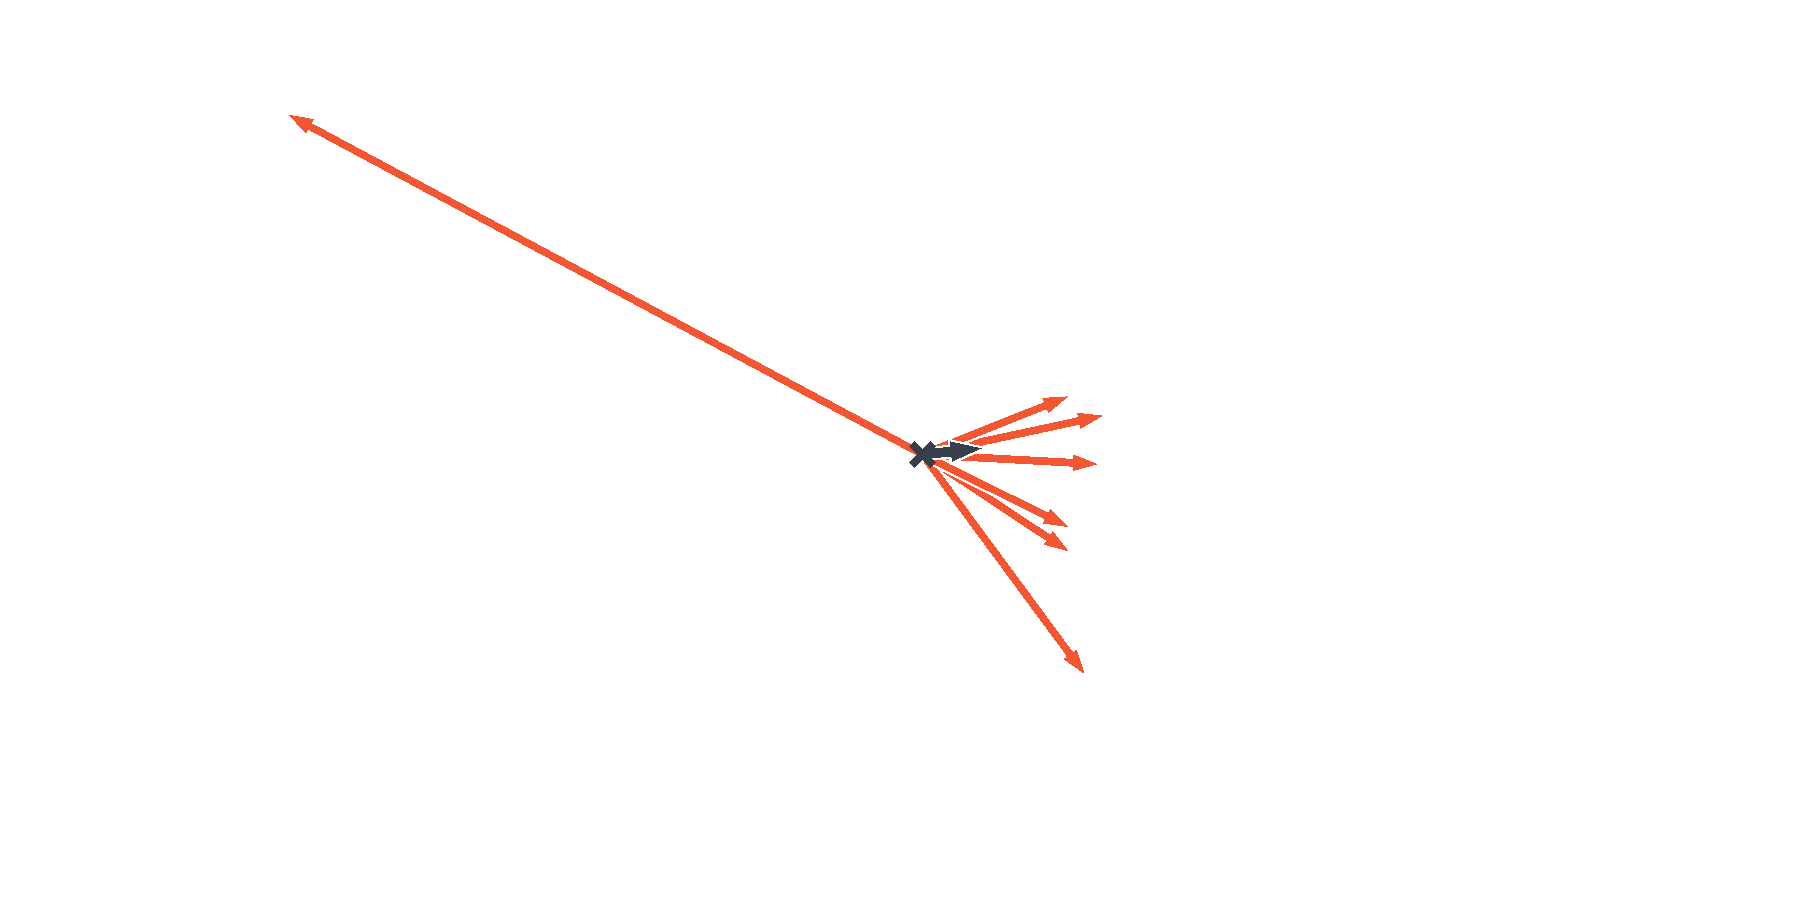
\includegraphics[width=\linewidth, trim={4.8cm 3.8cm 11.3cm 1.9cm}, clip]{../repos/backpack-paper/code/animations/differential-privacy/dp_frame_0}
    \caption{Individual gradients}\label{subfig:background::DifferentialPrivacy1}
  \end{subfigure}
  \begin{subfigure}{0.495\linewidth}
    % trim={<left> <lower> <right> <upper>}, clip
    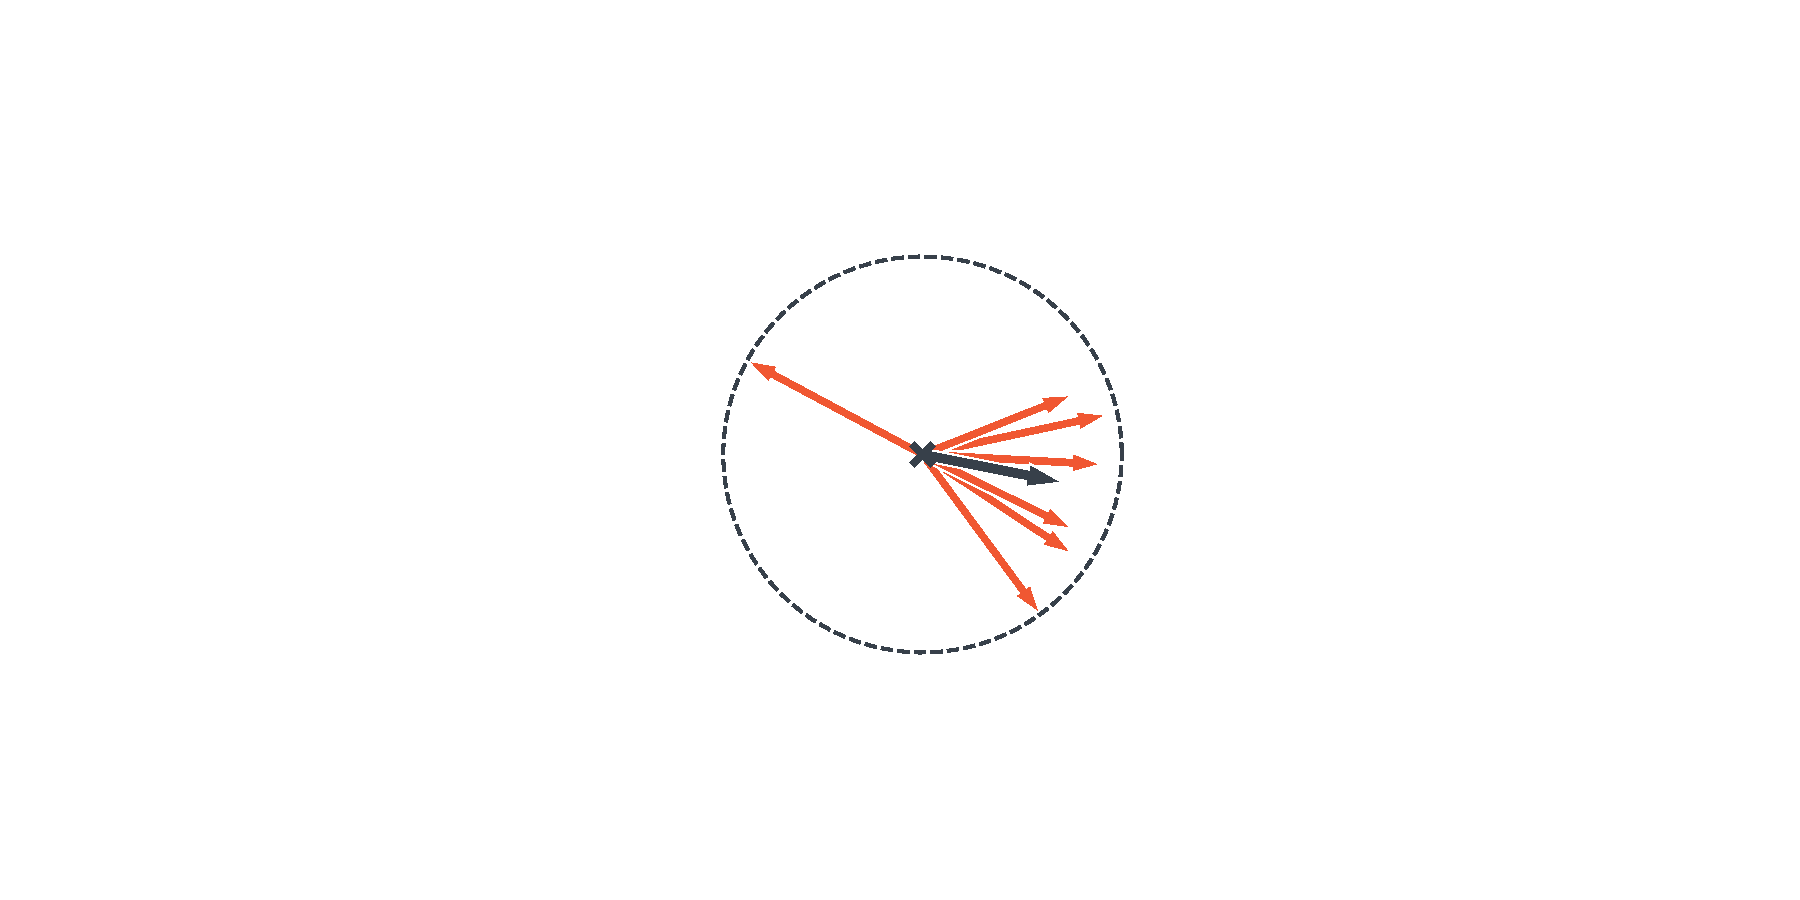
\includegraphics[width=\linewidth, trim={4.8cm 3.8cm 11.3cm 1.9cm}, clip]{../repos/backpack-paper/code/animations/differential-privacy/dp_frame_4}
    \caption{Clipped individual
      gradients}\label{subfig:background::DifferentialPrivacy2}
  \end{subfigure}
  \caption{\textbf{(Sketch) DP-SGD requires access to per-sample gradients.}
    \subfigref{subfig:background::DifferentialPrivacy1} The average gradient
    (black arrow) might be dominated by the per-sample gradients (orange arrows)
    of a small number of data. Adversaries might use this to extract potentially
    sensitive information about that data.
    \subfigref{subfig:background::DifferentialPrivacy2} Clipping per-sample
    gradients before averaging them limits the influence of individual data. The
    dashed circle's radius corresponds to the privacy threshold $C$.
  }\label{fig:background::DifferentialPrivacy}
\end{figure}

One prominent example for deep learning is differentially-private SGD
(DP-SGD)~\cite[Algorithm 1]{abadi2016deep}, which uses a negative average of
processed individual gradients over a mini-batch. To bound the influence of
individual data, per-sample gradients whose norm exceeds a specific threshold
$C$ are clipped back to norm $C$ (\Cref{fig:background::DifferentialPrivacy}),
\begin{align*}
  \vgtilde_n(\vtheta_t)
  =
  \frac{
  \vg_n(\vtheta_t)
  }{
  \max\left(
  1,
  \frac{\lVert \vg_n(\vtheta_t) \rVert_2}{C}
  \right)
  }\,.
\end{align*}
Gaussian noise of scale $\sigma$ is then added to each gradient,
\begin{align*}
  \vghat_n(\vtheta_t)
  =
  \vgtilde_n(\vtheta_t) + \vepsilon_n\,,
  \qquad
  \vepsilon_n \sim \gN(\vzero, {(\sigma C)}^2 \mI)\,.
\end{align*}
DP-SGD performs the update rule of SGD, with $\vg_n$ replaced by
$\vghat_n$,
\begin{align*}
  \vtheta_{t+1}
  =
  \vtheta_t
  -
  \eta_t
  \frac{1}{|\sB|}
  \sum_{(\vx_n,\vy_n) \in \sB}
  \vghat_n(\vtheta_t)\,.
\end{align*}
This requires access to per-sample gradient norms $\{\lVert \vg_n(\vtheta_t)
\rVert_2\}_{n}$.

\subsection{Importance Sampling}

\marginnote[*-22]{
  \begin{center}
    \pgfkeys{/pgfplots/BackPACKImportanceSamplingMNIST/.style={
    xmin = -0.02,
    xmax = 1.02,
    xtick={0, 1},
    xticklabels = {0, max},
    xlabel={$\lVert \nabla_{\vtheta}\ell_{n} \rVert_2$},
    scaled y ticks=real:50000,
    y tick label style={
      /pgf/number format/.cd,
      fixed,
      fixed zerofill,
      precision=2,
      /tikz/.cd
    },
    ytick scale label code/.code={$\cdot |\sD_{\text{train}}|$},
    ylabel = {},
    width = 1.15\linewidth,
    height = 0.9\linewidth,
    every axis plot/.append style={line width = 1.5pt},
    axis line style = black,
    tick pos = left,
    xtick align = inside,
    ytick align = inside,
    xmajorticks = true,
    ymajorticks = true,
    ylabel near ticks,
    xlabel near ticks,
    xticklabel style = {font = \footnotesize},
    xlabel style = {font = \footnotesize},
    yticklabel style = {font = \footnotesize},
    ylabel style = {font = \footnotesize},
    title style = {font = \footnotesize},
    grid = major,
    grid style = {dashed},
    legend cell align = left,
    legend style = {
      fill opacity = 0,
      text opacity = 0,
      draw opacity = 0,
      font = \footnotesize,
    },
  }
}

%%% Local Variables:
%%% mode: latex
%%% TeX-master: "../../thesis"
%%% End:

    \captionsetup[sub]{labelformat=parens}
    \begingroup
    \captionsetup{type=figure}
    \begin{subfigure}{\linewidth}
      \caption{Epoch 0, train accuracy 9.83\%}
      \vspace{-1ex}
      \pgfkeys{/pgfplots/zmystyle/.style={
          BackPACKImportanceSamplingMNIST,
          xlabel = \empty,
          xticklabel style = {opacity = 0},
        }
      }
      \tikzexternalenable
      % This file was created by tikzplotlib v0.9.0.
\begin{tikzpicture}

\definecolor{color0}{rgb}{0.941176470588235,0.341176470588235,0.196078431372549}

\begin{axis}[
axis line style={white!80!black},
legend cell align={left},
legend style={fill opacity=0.8, draw opacity=1, text opacity=1, draw=white!80!black},
tick pos=left,
x grid style={white!80!black},
xmin=0.180960892984677, xmax=1.03900186223882,
xtick style={color=gray},
xtick={0.1,0.2,0.3,0.4,0.5,0.6,0.7,0.8,0.9,1,1.1},
xticklabels={0.1,0.2,0.3,0.4,0.5,0.6,0.7,0.8,0.9,1.0,1.1},
y grid style={white!80!black},
ymin=0, ymax=3290.7,
ytick style={color=gray},
zmystyle
]
\draw[draw=white,fill=color0] (axis cs:0.219962755223502,0) rectangle (axis cs:0.235563500119032,4);
\addlegendimage{ybar,ybar legend,draw=white,fill=color0};
\addlegendentry{\ Epoch: 00, accuracy: 09.83\%}

\draw[draw=white,fill=color0] (axis cs:0.235563500119032,0) rectangle (axis cs:0.251164245014562,7);
\draw[draw=white,fill=color0] (axis cs:0.251164245014562,0) rectangle (axis cs:0.266764989910092,25);
\draw[draw=white,fill=color0] (axis cs:0.266764989910092,0) rectangle (axis cs:0.282365734805622,43);
\draw[draw=white,fill=color0] (axis cs:0.282365734805622,0) rectangle (axis cs:0.297966479701152,79);
\draw[draw=white,fill=color0] (axis cs:0.297966479701152,0) rectangle (axis cs:0.313567224596682,139);
\draw[draw=white,fill=color0] (axis cs:0.313567224596682,0) rectangle (axis cs:0.329167969492212,265);
\draw[draw=white,fill=color0] (axis cs:0.329167969492212,0) rectangle (axis cs:0.344768714387742,394);
\draw[draw=white,fill=color0] (axis cs:0.344768714387742,0) rectangle (axis cs:0.360369459283272,573);
\draw[draw=white,fill=color0] (axis cs:0.360369459283272,0) rectangle (axis cs:0.375970204178802,792);
\draw[draw=white,fill=color0] (axis cs:0.375970204178802,0) rectangle (axis cs:0.391570949074331,1008);
\draw[draw=white,fill=color0] (axis cs:0.391570949074332,0) rectangle (axis cs:0.407171693969862,1279);
\draw[draw=white,fill=color0] (axis cs:0.407171693969862,0) rectangle (axis cs:0.422772438865392,1519);
\draw[draw=white,fill=color0] (axis cs:0.422772438865392,0) rectangle (axis cs:0.438373183760921,1738);
\draw[draw=white,fill=color0] (axis cs:0.438373183760921,0) rectangle (axis cs:0.453973928656451,2090);
\draw[draw=white,fill=color0] (axis cs:0.453973928656451,0) rectangle (axis cs:0.469574673551981,2418);
\draw[draw=white,fill=color0] (axis cs:0.469574673551981,0) rectangle (axis cs:0.485175418447511,2540);
\draw[draw=white,fill=color0] (axis cs:0.485175418447511,0) rectangle (axis cs:0.500776163343041,2808);
\draw[draw=white,fill=color0] (axis cs:0.500776163343041,0) rectangle (axis cs:0.516376908238571,2924);
\draw[draw=white,fill=color0] (axis cs:0.516376908238571,0) rectangle (axis cs:0.531977653134101,3085);
\draw[draw=white,fill=color0] (axis cs:0.531977653134101,0) rectangle (axis cs:0.547578398029631,3063);
\draw[draw=white,fill=color0] (axis cs:0.547578398029631,0) rectangle (axis cs:0.563179142925161,3134);
\draw[draw=white,fill=color0] (axis cs:0.563179142925161,0) rectangle (axis cs:0.578779887820691,2925);
\draw[draw=white,fill=color0] (axis cs:0.578779887820691,0) rectangle (axis cs:0.594380632716221,2761);
\draw[draw=white,fill=color0] (axis cs:0.594380632716221,0) rectangle (axis cs:0.609981377611751,2560);
\draw[draw=white,fill=color0] (axis cs:0.609981377611751,0) rectangle (axis cs:0.625582122507281,2211);
\draw[draw=white,fill=color0] (axis cs:0.625582122507281,0) rectangle (axis cs:0.641182867402811,1927);
\draw[draw=white,fill=color0] (axis cs:0.641182867402811,0) rectangle (axis cs:0.656783612298341,1669);
\draw[draw=white,fill=color0] (axis cs:0.656783612298341,0) rectangle (axis cs:0.672384357193871,1476);
\draw[draw=white,fill=color0] (axis cs:0.672384357193871,0) rectangle (axis cs:0.687985102089401,1118);
\draw[draw=white,fill=color0] (axis cs:0.687985102089401,0) rectangle (axis cs:0.703585846984931,925);
\draw[draw=white,fill=color0] (axis cs:0.703585846984931,0) rectangle (axis cs:0.719186591880461,673);
\draw[draw=white,fill=color0] (axis cs:0.719186591880461,0) rectangle (axis cs:0.734787336775991,511);
\draw[draw=white,fill=color0] (axis cs:0.734787336775991,0) rectangle (axis cs:0.750388081671521,411);
\draw[draw=white,fill=color0] (axis cs:0.750388081671521,0) rectangle (axis cs:0.765988826567051,257);
\draw[draw=white,fill=color0] (axis cs:0.765988826567051,0) rectangle (axis cs:0.781589571462581,174);
\draw[draw=white,fill=color0] (axis cs:0.781589571462581,0) rectangle (axis cs:0.797190316358111,154);
\draw[draw=white,fill=color0] (axis cs:0.797190316358111,0) rectangle (axis cs:0.812791061253641,91);
\draw[draw=white,fill=color0] (axis cs:0.812791061253641,0) rectangle (axis cs:0.828391806149171,54);
\draw[draw=white,fill=color0] (axis cs:0.82839180614917,0) rectangle (axis cs:0.8439925510447,40);
\draw[draw=white,fill=color0] (axis cs:0.8439925510447,0) rectangle (axis cs:0.85959329594023,17);
\draw[draw=white,fill=color0] (axis cs:0.85959329594023,0) rectangle (axis cs:0.87519404083576,20);
\draw[draw=white,fill=color0] (axis cs:0.87519404083576,0) rectangle (axis cs:0.89079478573129,9);
\draw[draw=white,fill=color0] (axis cs:0.89079478573129,0) rectangle (axis cs:0.90639553062682,4);
\draw[draw=white,fill=color0] (axis cs:0.90639553062682,0) rectangle (axis cs:0.92199627552235,2);
\draw[draw=white,fill=color0] (axis cs:0.92199627552235,0) rectangle (axis cs:0.93759702041788,1);
\draw[draw=white,fill=color0] (axis cs:0.93759702041788,0) rectangle (axis cs:0.95319776531341,2);
\draw[draw=white,fill=color0] (axis cs:0.95319776531341,0) rectangle (axis cs:0.96879851020894,0);
\draw[draw=white,fill=color0] (axis cs:0.96879851020894,0) rectangle (axis cs:0.98439925510447,0);
\draw[draw=white,fill=color0] (axis cs:0.98439925510447,0) rectangle (axis cs:1,1);
\end{axis}

\end{tikzpicture}

      \tikzexternaldisable
      \vspace{-6ex}
    \end{subfigure}
    \begin{subfigure}{\linewidth}
      \caption{Epoch 2, train accuracy 83.4\%}
      \vspace{-1ex}
      \pgfkeys{/pgfplots/zmystyle/.style={
          BackPACKImportanceSamplingMNIST,
          xlabel = \empty,
          xticklabel style = {opacity = 0},
        }
      }
      \tikzexternalenable
      % This file was created by tikzplotlib v0.9.0.
\begin{tikzpicture}

\definecolor{color0}{rgb}{0.941176470588235,0.341176470588235,0.196078431372549}

\begin{axis}[
axis line style={white!80!black},
legend cell align={left},
legend style={fill opacity=0.8, draw opacity=1, text opacity=1, draw=white!80!black},
tick pos=left,
x grid style={white!80!black},
xmin=-0.0235874482194031, xmax=1.04874225943902,
xtick style={color=gray},
xtick={-0.2,0,0.2,0.4,0.6,0.8,1,1.2},
xticklabels={−0.2,0.0,0.2,0.4,0.6,0.8,1.0,1.2},
y grid style={white!80!black},
ymin=0, ymax=3099.6,
ytick style={color=gray},
zmystyle
]
\draw[draw=white,fill=color0] (axis cs:0.0251548112196161,0) rectangle (axis cs:0.0446517149952238,90);
\addlegendimage{ybar,ybar legend,draw=white,fill=color0};
\addlegendentry{\ Epoch: 02, accuracy: 83.40\%}

\draw[draw=white,fill=color0] (axis cs:0.0446517149952238,0) rectangle (axis cs:0.0641486187708315,293);
\draw[draw=white,fill=color0] (axis cs:0.0641486187708315,0) rectangle (axis cs:0.0836455225464392,611);
\draw[draw=white,fill=color0] (axis cs:0.0836455225464392,0) rectangle (axis cs:0.103142426322047,1523);
\draw[draw=white,fill=color0] (axis cs:0.103142426322047,0) rectangle (axis cs:0.122639330097655,1968);
\draw[draw=white,fill=color0] (axis cs:0.122639330097655,0) rectangle (axis cs:0.142136233873262,1998);
\draw[draw=white,fill=color0] (axis cs:0.142136233873262,0) rectangle (axis cs:0.16163313764887,1973);
\draw[draw=white,fill=color0] (axis cs:0.16163313764887,0) rectangle (axis cs:0.181130041424478,2001);
\draw[draw=white,fill=color0] (axis cs:0.181130041424478,0) rectangle (axis cs:0.200626945200085,2081);
\draw[draw=white,fill=color0] (axis cs:0.200626945200085,0) rectangle (axis cs:0.220123848975693,2047);
\draw[draw=white,fill=color0] (axis cs:0.220123848975693,0) rectangle (axis cs:0.239620752751301,2217);
\draw[draw=white,fill=color0] (axis cs:0.239620752751301,0) rectangle (axis cs:0.259117656526908,2397);
\draw[draw=white,fill=color0] (axis cs:0.259117656526908,0) rectangle (axis cs:0.278614560302516,2682);
\draw[draw=white,fill=color0] (axis cs:0.278614560302516,0) rectangle (axis cs:0.298111464078124,2769);
\draw[draw=white,fill=color0] (axis cs:0.298111464078124,0) rectangle (axis cs:0.317608367853731,2952);
\draw[draw=white,fill=color0] (axis cs:0.317608367853731,0) rectangle (axis cs:0.337105271629339,2754);
\draw[draw=white,fill=color0] (axis cs:0.337105271629339,0) rectangle (axis cs:0.356602175404947,2654);
\draw[draw=white,fill=color0] (axis cs:0.356602175404947,0) rectangle (axis cs:0.376099079180554,2566);
\draw[draw=white,fill=color0] (axis cs:0.376099079180554,0) rectangle (axis cs:0.395595982956162,2335);
\draw[draw=white,fill=color0] (axis cs:0.395595982956162,0) rectangle (axis cs:0.41509288673177,2063);
\draw[draw=white,fill=color0] (axis cs:0.41509288673177,0) rectangle (axis cs:0.434589790507377,1800);
\draw[draw=white,fill=color0] (axis cs:0.434589790507377,0) rectangle (axis cs:0.454086694282985,1570);
\draw[draw=white,fill=color0] (axis cs:0.454086694282985,0) rectangle (axis cs:0.473583598058593,1361);
\draw[draw=white,fill=color0] (axis cs:0.473583598058593,0) rectangle (axis cs:0.4930805018342,1056);
\draw[draw=white,fill=color0] (axis cs:0.4930805018342,0) rectangle (axis cs:0.512577405609808,891);
\draw[draw=white,fill=color0] (axis cs:0.512577405609808,0) rectangle (axis cs:0.532074309385416,730);
\draw[draw=white,fill=color0] (axis cs:0.532074309385416,0) rectangle (axis cs:0.551571213161023,567);
\draw[draw=white,fill=color0] (axis cs:0.551571213161023,0) rectangle (axis cs:0.571068116936631,437);
\draw[draw=white,fill=color0] (axis cs:0.571068116936631,0) rectangle (axis cs:0.590565020712239,347);
\draw[draw=white,fill=color0] (axis cs:0.590565020712239,0) rectangle (axis cs:0.610061924487846,290);
\draw[draw=white,fill=color0] (axis cs:0.610061924487846,0) rectangle (axis cs:0.629558828263454,207);
\draw[draw=white,fill=color0] (axis cs:0.629558828263454,0) rectangle (axis cs:0.649055732039062,195);
\draw[draw=white,fill=color0] (axis cs:0.649055732039062,0) rectangle (axis cs:0.66855263581467,138);
\draw[draw=white,fill=color0] (axis cs:0.668552635814669,0) rectangle (axis cs:0.688049539590277,106);
\draw[draw=white,fill=color0] (axis cs:0.688049539590277,0) rectangle (axis cs:0.707546443365885,67);
\draw[draw=white,fill=color0] (axis cs:0.707546443365885,0) rectangle (axis cs:0.727043347141493,54);
\draw[draw=white,fill=color0] (axis cs:0.727043347141493,0) rectangle (axis cs:0.7465402509171,35);
\draw[draw=white,fill=color0] (axis cs:0.7465402509171,0) rectangle (axis cs:0.766037154692708,35);
\draw[draw=white,fill=color0] (axis cs:0.766037154692708,0) rectangle (axis cs:0.785534058468316,13);
\draw[draw=white,fill=color0] (axis cs:0.785534058468316,0) rectangle (axis cs:0.805030962243923,16);
\draw[draw=white,fill=color0] (axis cs:0.805030962243923,0) rectangle (axis cs:0.824527866019531,14);
\draw[draw=white,fill=color0] (axis cs:0.824527866019531,0) rectangle (axis cs:0.844024769795139,4);
\draw[draw=white,fill=color0] (axis cs:0.844024769795139,0) rectangle (axis cs:0.863521673570746,5);
\draw[draw=white,fill=color0] (axis cs:0.863521673570746,0) rectangle (axis cs:0.883018577346354,2);
\draw[draw=white,fill=color0] (axis cs:0.883018577346354,0) rectangle (axis cs:0.902515481121962,2);
\draw[draw=white,fill=color0] (axis cs:0.902515481121962,0) rectangle (axis cs:0.922012384897569,1);
\draw[draw=white,fill=color0] (axis cs:0.922012384897569,0) rectangle (axis cs:0.941509288673177,0);
\draw[draw=white,fill=color0] (axis cs:0.941509288673177,0) rectangle (axis cs:0.961006192448785,0);
\draw[draw=white,fill=color0] (axis cs:0.961006192448785,0) rectangle (axis cs:0.980503096224392,2);
\draw[draw=white,fill=color0] (axis cs:0.980503096224392,0) rectangle (axis cs:1,1);
\end{axis}

\end{tikzpicture}

      \tikzexternaldisable
      \vspace{-6ex}
    \end{subfigure}
    \begin{subfigure}{\linewidth}
      \caption{Epoch 49, train accuracy 90.5\%}
      \vspace{-1ex}
      \pgfkeys{/pgfplots/zmystyle/.style={
          BackPACKImportanceSamplingMNIST,
        }
      }
      \tikzexternalenable
      % This file was created by tikzplotlib v0.9.0.
\begin{tikzpicture}

\definecolor{color0}{rgb}{0.941176470588235,0.341176470588235,0.196078431372549}

\begin{axis}[
axis line style={white!80!black},
legend cell align={left},
legend style={fill opacity=0.8, draw opacity=1, text opacity=1, draw=white!80!black},
tick pos=left,
x grid style={white!80!black},
xmin=-0.0499953146370904, xmax=1.04999977688748,
xtick style={color=gray},
xtick={-0.2,0,0.2,0.4,0.6,0.8,1,1.2},
xticklabels={−0.2,0.0,0.2,0.4,0.6,0.8,1.0,1.2},
y grid style={white!80!black},
ymin=0, ymax=20526.45,
ytick style={color=gray},
zmystyle
]
\draw[draw=white,fill=color0] (axis cs:4.46225039008562e-06,0) rectangle (axis cs:0.0200043730053823,19549);
\addlegendimage{ybar,ybar legend,draw=white,fill=color0};
\addlegendentry{\ Epoch: 49, accuracy: 90.49\%}

\draw[draw=white,fill=color0] (axis cs:0.0200043730053823,0) rectangle (axis cs:0.0400042837603745,7018);
\draw[draw=white,fill=color0] (axis cs:0.0400042837603745,0) rectangle (axis cs:0.0600041945153667,4100);
\draw[draw=white,fill=color0] (axis cs:0.0600041945153667,0) rectangle (axis cs:0.0800041052703589,2853);
\draw[draw=white,fill=color0] (axis cs:0.0800041052703589,0) rectangle (axis cs:0.100004016025351,2112);
\draw[draw=white,fill=color0] (axis cs:0.100004016025351,0) rectangle (axis cs:0.120003926780343,1752);
\draw[draw=white,fill=color0] (axis cs:0.120003926780343,0) rectangle (axis cs:0.140003837535335,1514);
\draw[draw=white,fill=color0] (axis cs:0.140003837535335,0) rectangle (axis cs:0.160003748290328,1212);
\draw[draw=white,fill=color0] (axis cs:0.160003748290328,0) rectangle (axis cs:0.18000365904532,1032);
\draw[draw=white,fill=color0] (axis cs:0.18000365904532,0) rectangle (axis cs:0.200003569800312,866);
\draw[draw=white,fill=color0] (axis cs:0.200003569800312,0) rectangle (axis cs:0.220003480555304,810);
\draw[draw=white,fill=color0] (axis cs:0.220003480555304,0) rectangle (axis cs:0.240003391310296,694);
\draw[draw=white,fill=color0] (axis cs:0.240003391310296,0) rectangle (axis cs:0.260003302065289,661);
\draw[draw=white,fill=color0] (axis cs:0.260003302065289,0) rectangle (axis cs:0.280003212820281,594);
\draw[draw=white,fill=color0] (axis cs:0.280003212820281,0) rectangle (axis cs:0.300003123575273,537);
\draw[draw=white,fill=color0] (axis cs:0.300003123575273,0) rectangle (axis cs:0.320003034330265,521);
\draw[draw=white,fill=color0] (axis cs:0.320003034330265,0) rectangle (axis cs:0.340002945085257,462);
\draw[draw=white,fill=color0] (axis cs:0.340002945085257,0) rectangle (axis cs:0.36000285584025,415);
\draw[draw=white,fill=color0] (axis cs:0.36000285584025,0) rectangle (axis cs:0.380002766595242,391);
\draw[draw=white,fill=color0] (axis cs:0.380002766595242,0) rectangle (axis cs:0.400002677350234,384);
\draw[draw=white,fill=color0] (axis cs:0.400002677350234,0) rectangle (axis cs:0.420002588105226,341);
\draw[draw=white,fill=color0] (axis cs:0.420002588105226,0) rectangle (axis cs:0.440002498860218,325);
\draw[draw=white,fill=color0] (axis cs:0.440002498860218,0) rectangle (axis cs:0.460002409615211,271);
\draw[draw=white,fill=color0] (axis cs:0.460002409615211,0) rectangle (axis cs:0.480002320370203,261);
\draw[draw=white,fill=color0] (axis cs:0.480002320370203,0) rectangle (axis cs:0.500002231125195,230);
\draw[draw=white,fill=color0] (axis cs:0.500002231125195,0) rectangle (axis cs:0.520002141880187,188);
\draw[draw=white,fill=color0] (axis cs:0.520002141880187,0) rectangle (axis cs:0.54000205263518,160);
\draw[draw=white,fill=color0] (axis cs:0.54000205263518,0) rectangle (axis cs:0.560001963390172,123);
\draw[draw=white,fill=color0] (axis cs:0.560001963390172,0) rectangle (axis cs:0.580001874145164,129);
\draw[draw=white,fill=color0] (axis cs:0.580001874145164,0) rectangle (axis cs:0.600001784900156,92);
\draw[draw=white,fill=color0] (axis cs:0.600001784900156,0) rectangle (axis cs:0.620001695655148,73);
\draw[draw=white,fill=color0] (axis cs:0.620001695655148,0) rectangle (axis cs:0.64000160641014,67);
\draw[draw=white,fill=color0] (axis cs:0.64000160641014,0) rectangle (axis cs:0.660001517165133,50);
\draw[draw=white,fill=color0] (axis cs:0.660001517165133,0) rectangle (axis cs:0.680001427920125,32);
\draw[draw=white,fill=color0] (axis cs:0.680001427920125,0) rectangle (axis cs:0.700001338675117,26);
\draw[draw=white,fill=color0] (axis cs:0.700001338675117,0) rectangle (axis cs:0.720001249430109,31);
\draw[draw=white,fill=color0] (axis cs:0.720001249430109,0) rectangle (axis cs:0.740001160185101,15);
\draw[draw=white,fill=color0] (axis cs:0.740001160185102,0) rectangle (axis cs:0.760001070940094,9);
\draw[draw=white,fill=color0] (axis cs:0.760001070940094,0) rectangle (axis cs:0.780000981695086,7);
\draw[draw=white,fill=color0] (axis cs:0.780000981695086,0) rectangle (axis cs:0.800000892450078,6);
\draw[draw=white,fill=color0] (axis cs:0.800000892450078,0) rectangle (axis cs:0.82000080320507,1);
\draw[draw=white,fill=color0] (axis cs:0.82000080320507,0) rectangle (axis cs:0.840000713960062,1);
\draw[draw=white,fill=color0] (axis cs:0.840000713960062,0) rectangle (axis cs:0.860000624715055,0);
\draw[draw=white,fill=color0] (axis cs:0.860000624715055,0) rectangle (axis cs:0.880000535470047,2);
\draw[draw=white,fill=color0] (axis cs:0.880000535470047,0) rectangle (axis cs:0.900000446225039,0);
\draw[draw=white,fill=color0] (axis cs:0.900000446225039,0) rectangle (axis cs:0.920000356980031,0);
\draw[draw=white,fill=color0] (axis cs:0.920000356980031,0) rectangle (axis cs:0.940000267735023,2);
\draw[draw=white,fill=color0] (axis cs:0.940000267735023,0) rectangle (axis cs:0.960000178490016,0);
\draw[draw=white,fill=color0] (axis cs:0.960000178490016,0) rectangle (axis cs:0.980000089245008,0);
\draw[draw=white,fill=color0] (axis cs:0.980000089245008,0) rectangle (axis cs:1,1);
\end{axis}

\end{tikzpicture}

      \tikzexternaldisable
      \vspace{-2ex}
    \end{subfigure}
    \endgroup
    \captionof{figure}{\textbf{Importance distribution of samples during
        training.} Importance is measured by individual gradient $L_{2}$ norms,
      computed with \backpack (\Cref{chap:backpack}). As training proceeds and
      more examples are correctly classified and become ``unimportant''.
      Details: logistic regression on \mnist, trained with \sgd, $|\sB| = 128$,
      and learning rate $0.005$.}\label{fig:background::SquaredL2Norms}
  \end{center}
}

A hypothesis about learning in ML is that the model first learns to correctly
predict ``easy'' examples. Only in later phases are the ``difficult'' examples
learned. Using these harder examples more frequently for training might help
speed up the learning procedure. Put differently, some data matter more at
certain stages of training than other, which is quantified through a measure of
importance. Importance sampling realizes this idea of selecting important data
more frequently. It does so by adapting the sampling procedure for mini-batches
to reduce the gradient variance, which beneficially influences the convergence
of stochastic first-order methods like \sgd, and therefore speeds up training. A
common strategy is to weight the importance of samples by the per-sample $L_2$
norm
(\Cref{eq:background::importanceSamplingOptimalDistribution,fig:background::SquaredL2Norms}).

As a starting point to see how the sampling procedure affects optimization,
consider the generalization of uniform sampling from
\Cref{sec:background::MiniBatching} for $|\sB| = 1$. At training iteration $t$,
a sample $n_t\sim p_t(n_t)$ is drawn from a current sampling distribution
$p_t(n_t)$ over $\{1, \dots, |\sD|\}$. \sgd with a learning rate $\eta$ uses the
unbiased gradient estimator\sidenote[][0\baselineskip]{%
  For uniform sampling $p_{t}(n_{t}) = \nicefrac{1}{|\sD|}$, which is the most
  common case in practice, the scaling factor cancels and yields the commonly
  used gradient estimator that would be used by ``normal'' \sgd with $|\sB| =
  1$.%
}
\begin{subequations}
  \begin{align}\label{eq:background::gradientEstimator}
    \vghat_{n_t}(\vtheta_t)
    &:=
      \frac{1}{|\sD| p_t(n_t)}
      \grad{\vtheta_t}\ell_{n_t}(\vtheta_t)
      \shortintertext{with}
      \E_{n_t \sim p_t(n_t)}\left[ \vghat_{n_t}(\vtheta_t) \right]
    &=
      \frac{1}{|\sD|} \sum_{(\vx_n, \vy_n) \in \sD}
      \grad{\vtheta_t} \ell_{n_t}(\vtheta_t)
      = \vg_{\sD}(\vtheta_t)
      \shortintertext{to update the parameters}
      \label{eq:background::gradientDescentSampled}
      \vtheta_{t+1} &= \vtheta_t - \eta \vghat_{n_t}(\vtheta_{t})\,.
  \end{align}
\end{subequations}
Using a non-uniform distribution over stochastic gradients would introduce bias
in the update, so in importance sampling the samples are weighted by their
probability of being selected to undo the bias. The distribution can then be
tuned to minimize the variance of the estimator and improve performance: one can
assess convergence of \Cref{eq:background::gradientDescentSampled} through the
progress towards the minimizer $\vtheta_{\star}$ in terms of squared $L_2$
distance~\cite{wang2017accelerating,katharopoulos2018samples},
\begin{subequations}
  \begin{align}
    \lVert \vtheta_{t} - \vtheta_{\star} \rVert_2^{2}
    -
    \lVert \vtheta_{t+1} - \vtheta_{\star} \rVert_2^{2}\,.
  \end{align}
  In expectation, this measure of convergence depends on the gradient estimator's
  variance (more specifically, its trace),
  \begin{align}
    \begin{split}
      \E_{n_t}
      &\left[
        \lVert \vtheta_{t} - \vtheta_{\star} \rVert_2^2
        -
        \lVert \vtheta_{t+1} - \vtheta_{\star} \rVert_2^2
        \right]
      \\
      &=
        \E_{n_t}\left[
        \lVert \vtheta_{t} - \vtheta_{\star} \rVert_2^{2}
        -
        \lVert \vtheta_{t} - \vtheta_{\star} - \eta \vghat_{n_t}  \rVert_2^{2}
        \right]
      \\
      &=
        \E_{n_t}\left[
        2 \eta \left(
        \vtheta_{t} - \vtheta_{\star}
        \right)^{\top} \vghat_{n_t}
        - \eta^2 \vghat_{n_t}^{\top} \vghat_{n_t}
        \right]
      \\
      &=
        2 \eta \left(
        \vtheta_{t} - \vtheta_{\star}
        \right)^{\top}
        \vg_{\sD}
        -
        \eta^2 \E_{n_t}\left[
        \lVert \vghat_{n_t} \rVert_2^2
        \right]
      \\
      &=
        2 \eta \left(
        \vtheta_{t} - \vtheta_{\star}
        \right)^{\top}
        \vg_{\sD}
        - \eta^2 \lVert \vg_{\sD} \rVert_2^2
        -
        \eta^2 \E_{n_t}\left[
        \lVert \vghat_{n_t} - \vg_{\sD} \rVert_2^2
        \right]
      \\
      &=
        2 \eta \left(
        \vtheta_{t} - \vtheta_{\star}
        \right)^{\top}
        \vg_{\sD}
        - \eta^2 \lVert \vg_{\sD} \rVert_2^2
        -
        \eta^2 \Tr\left\{
        \Var_{n_t}\left[\vghat_{n_t}
        \right]\right\}
    \end{split}
  \end{align}
\end{subequations}
For what follows, the intuition is that sampling affects convergence through the
variance term, and minimizing this term improves convergence. Hence, the goal is
to identify the optimal sampling via
\begin{align}\label{ex:background::findOptimalSamplingDistribution}
  \minimize_{\substack{p_t(n_t) \\ \sum_{n=1}^{|\sD|} p_t(n) = 1}}
  \Tr\left\{
  \Var_{n_t}\left[\vghat_{n_t}
  \right]\right\}
  \quad
  \Leftrightarrow
  \quad
  \minimize_{\substack{p_t(n_t) \\ \sum_{n=1}^{|\sD|} p_t(n) = 1}}
  \E_{n_t}
  \left[
  \lVert
  \vghat_{n_t}
  \rVert_2^2
  \right]
\end{align}
The solution, outlined in \Cref{ex:background::importanceSamplingDerivation}, is
\begin{align}
  \label{eq:background::importanceSamplingOptimalDistribution}
  p_t(n_t)
  =
  \frac{
  \lVert \grad{\vtheta_t}\ell_{n_t}(\vtheta_t) \rVert_2
  }{
  \sum_{n=1}^{|\sD|} \lVert \ell_{n}(\vtheta_t) \rVert_2
  }\,.
\end{align}
%
and
\marginnote[*-31]{%
  \begin{remark}[\textbf{Optimal sampling
      distribution~\cite{needell2014stochastic,zhao2015stochastic}}]\label{ex:background::importanceSamplingDerivation}
    (The iteration index $t$ is suppressed for brevity) To derive
    \Cref{eq:background::importanceSamplingOptimalDistribution}, one
    incorporates the constraint in
    \Cref{ex:background::findOptimalSamplingDistribution} via a Lagrange
    multiplier $\mu \in \sR$, writing $p(n)$ as $|\sD|$-dimensional vector
    $\vp$. Expanding $\vghat$ with \Cref{eq:background::gradientEstimator} leads
    to,
    \begin{align*}
      A(\vp, \mu)
      &:=
        \frac{1}{|\sD|^2}
        \sum_{n=1}^{|\sD|}
        \frac{
        \lVert \grad{\vtheta}\ell_n(\vtheta)\rVert_2^2
        }{
        \evp_n
        }
      \\
      &\phantom{= } \
        +
        \mu
        \left(
        \sum_{n=1}^{|\sD|}
        \evp_n
        -1
        \right)\,.
    \end{align*}
    Setting the $\evp_n$-derivative of that to zero yields
    \begin{align*}
      \grad{\evp_n} A(\vp, \mu)
      &=
        -
        \frac{
        \lVert \grad{\vtheta}\ell_n(\vtheta)\rVert_2^2
        }{
        |\sD|^2
        \evp_n^2
        }
        + \mu
        \overset{!}{=} 0
      \\
      \implies
      \quad
      \evp_n
      &=
        \frac{
        \lVert \grad{\vtheta}\ell_n(\vtheta)\rVert_2
        }{
        \sqrt{\mu}
        }\,,
    \end{align*}
    using that all elements $\evp_n \in (0; 1)$ of $\vp$. Inserting into
    $A$ gives
    \begin{align*}
      A(\mu)
      =
      \frac{2}{|\sD|}
      \sqrt{\mu}
      \sum_{n=1}^{|\sD|}
      \lVert \grad{\vtheta}\ell_n(\vtheta)\rVert_2
      -
      \mu
    \end{align*}
    Setting the $\mu$-derivative to zero yields
    \begin{align*}
      \grad{\mu}A(\mu)
      &=
        \frac{1}{|\sD| \sqrt{\mu}}
        \sum_{n=1}^{|\sD|}
        \lVert \grad{\vtheta}\ell_n(\vtheta)\rVert_2
        - 1
        \overset{!}{=} 0
      \\
      \implies
      \quad
      \sqrt{\mu}
      &=
        \frac{1}{|\sD|}
        \sum_{n=1}^{|\sD|}
        \lVert \grad{\vtheta}\ell_n(\vtheta)\rVert_2
    \end{align*}
    This then leads to
    \begin{align*}
      \evp_n
      =
      \frac{
      \lVert \grad{\vtheta}\ell_n(\vtheta)\rVert_2
      }{
      \sum_{n=1}^{|\sD|}
      \lVert \grad{\vtheta}\ell_n(\vtheta)\rVert_2
      }
    \end{align*}
    which equals \Cref{eq:background::importanceSamplingOptimalDistribution}
    when switching back notation and introducing the iteration count.
  \end{remark}
} %
depends on individual gradient $L_2$ norms in the entire dataset. Samples with
higher importance, \ie gradient norm, are drawn more frequently. Because
computing the sampling distribution requires a sweep over all data, practical
versions further approximate
\Cref{eq:background::importanceSamplingOptimalDistribution}, \eg by relaxing the
optimization through bounds that are easier to compute, or updating the
distribution only every few iterations~\cite{katharopoulos2018samples}.

%%% Local Variables:
%%% mode: latex
%%% TeX-master: "../thesis"
%%% End:


%%% Local Variables:
%%% mode: latex
%%% TeX-master: "../thesis"
%%% End: